%%%%%%%%%%%%%%%%%%%%%%%%%%%%%%%%%%%%%%%%%%%%%%%%%%%%%%%%%%%%%%%%%%%%%%%%%%%%%%%%%%%%%%%%%%%%%%%%%%%%%%%%%%%%%%%%%%%%%%%%%%%%%%%%%%%%%%%%%%%%%%%%%%%%%%%%%%%
% This is just an example/guide for you to refer to when submitting manuscripts to Frontiers, it is not mandatory to use Frontiers .cls files nor frontiers.tex  %
% This will only generate the Manuscript, the final article will be typeset by Frontiers after acceptance.   
%                                              %
%                                                                                                                                                         %
% When submitting your files, remember to upload this *tex file, the pdf generated with it, the *bib file (if bibliography is not within the *tex) and all the figures.
%%%%%%%%%%%%%%%%%%%%%%%%%%%%%%%%%%%%%%%%%%%%%%%%%%%%%%%%%%%%%%%%%%%%%%%%%%%%%%%%%%%%%%%%%%%%%%%%%%%%%%%%%%%%%%%%%%%%%%%%%%%%%%%%%%%%%%%%%%%%%%%%%%%%%%%%%%%

%%% Version 3.4 Generated 2018/06/15 %%%
%%% You will need to have the following packages installed: datetime, fmtcount, etoolbox, fcprefix, which are normally inlcuded in WinEdt. %%%
%%% In http://www.ctan.org/ you can find the packages and how to install them, if necessary. %%%
%%%  NB logo1.jpg is required in the path in order to correctly compile front page header %%%

\documentclass[utf8]{frontiersSCNS} % for Science, Engineering and Humanities and Social Sciences articles
%\documentclass[utf8]{frontiersHLTH} % for Health articles
%\documentclass[utf8]{frontiersFPHY} % for Physics and Applied Mathematics and Statistics articles

%\setcitestyle{square} % for Physics and Applied Mathematics and Statistics articles
\usepackage{url,hyperref,lineno,microtype,subcaption}
\usepackage[onehalfspacing]{setspace}
\linenumbers

\graphicspath{{./figures/}}

\def\keyFont{\fontsize{8}{11}\helveticabold }
%%%%%%%%%%%%%%%%%%%%%%%%%%%%%%%%%%%%%%
%%%%%%%%%%%%%%%%%%%%%%%%%%%%%%%%%%%%%%

\def\firstAuthorLast{Fabian Schubert and Claudius Gros} %use et al 
%only if is more than 1 author

\def\Authors{Fabian Schubert\,$^{1,*}$ and Claudius Gros\,$^{1}$}

% Affiliations should be keyed to the author's name with superscript 
%numbers and be listed as follows: Laboratory, Institute, Department, 
%Organization, City, State abbreviation (USA, Canada, Australia), and 
%Country (without detailed address information such as city zip codes 
%or street names).
% If one of the authors has a change of address, list the new address 
%below the correspondence details using a superscript symbol and use 
%the same symbol to indicate the author in the author list.

\def\Address{$^{1}$Institute for Theoretical Physics, 
	Goethe University Frankfurt am Main, Germany}

% The Corresponding Author should be marked with an asterisk
% Provide the exact contact address (this time including street name 
%and city zip code) and email of the corresponding author

\def\corrAuthor{Institute for Theoretical Physics\\
	Goethe University Frankfurt am Main\\
	Max-von-Laue-Str. 1\\
	60438 Frankfurt am Main, Germany}

\def\corrEmail{fschubert@itp.uni-frankfurt.de}

\begin{document}
\onecolumn
\firstpage{1}

\title[Running Title]{Nonlinear Dendritic Coincidence Detection for Supervised Learning} 

\author[\firstAuthorLast ]{\Authors} %This field will be automatically populated
\address{} %This field will be automatically populated
\correspondance{} %This field will be automatically populated

\extraAuth{}% If there are more than 1 corresponding author, comment this line and uncomment the next one.
%\extraAuth{corresponding Author2 \\ Laboratory X2, Institute X2, Department X2, Organization X2, Street X2, City X2 , State XX2 (only USA, Canada and Australia), Zip Code2, X2 Country X2, email2@uni2.edu}


\maketitle


\begin{abstract}

Cortical pyramidal neurons have a complex 
dendritic anatomy, whose function is an active 
field of scientific research. In particular, 
the segregation between its soma and the apical 
dendritic tree is believed to play an active 
role in processing feed-forward sensory 
information and top-down or feedback signals. 
In this work, we use a simple two-compartment 
model accounting for the nonlinear interactions 
between basal and apical input streams and show 
that a simple Hebbian learning rule in the basal 
compartment allows the neuron to align its basal 
input to a target signal in the apical compartment. 
We show that this learning process, termed 
coincidence detection, is robust against strong 
distractions in the basal input space and 
demonstrate its effectiveness in a linear 
classification task.

\tiny
 \keyFont{ \section{Keywords:} Dendrites, Pyramidal Neuron, Plasticity, 
 	Coincidence Detection, Supervised Learning}
\end{abstract}

%---------------------------------------%
\section{Introduction}
\label{sect:introduction}
%---------------------------------------%

In recent years, a growing body of research has addressed the 
functional implications of the distinct physiology and anatomy of 
cortical pyramidal neurons \citep{Spruston2008,Hay2011,Ramaswamy2015}. 
In particular, on the theoretical side,
we saw a paradigm shift from treating neurons as point-like electrical
structures towards embracing the entire dendritic structure 
\citep{Larkum2009,Poirazi2009,Shai2015}. This was 
mostly due to the fact that experimental work 
uncovered dynamical properties of pyramidal neuronal
cells that simply could not be accounted for by point models
\citep{Spruston1995,Hausser2000}.

An important finding is that the apical dendritic tree of
cortical pyramidal neurons can act as a separate nonlinear synaptic 
integration zone \citep{Spruston2008,Branco2011}. 
Under certain conditions, a dendritic $\rm Ca^{2+}$ spike
can be elicited that propagates towards the soma, causing rapid, bursting
spiking activity. One of the cases in which dendritic spiking can occur
was termed `backpropagation-activated $\rm Ca^{2+}$ spike firing' 
(`BAC firing'): A single somatic spike can backpropagate towards the apical
spike initiation zone, in turn significantly facilitating the initiation of 
a dendritic spike \citep{Stuart2001,Spruston2008,Larkum2013}. 
This reciprocal coupling is believed to act as a form of
coincidence detection: If apical and basal synaptic input co-occurs, the 
neuron can respond with a rapid burst of spiking activity. 
The firing rate of these temporal bursts exceeds the firing 
rate that is maximally achievable under basal synaptic input alone, 
therefore representing a form of temporal coincidence
detection between apical and basal input.

Naturally, these mechanisms also affect plasticity and thus learning
within the cortex \citep{Sjoestroem2006,Ebner2019}. 
While the interplay between basal and apical stimulation and
its effect on synaptic efficacies is subject to ongoing research, 
there is evidence that BAC-firing tends to shift plasticity 
towards long-term potentiation (LTP) \citep{Letzkus2006}. 
Thus, coincidence between basal and apical input appears 
to also gate synaptic plasticity.

In a supervised learning scheme, where the top down input
arriving at the apical compartment acts as the teaching signal,
the most straight-forward learning rule for the basal synaptic
weights would be derived from an appropriate loss function,
such as a mean square error, based on the difference between 
basal and apical input, i.e.\ $I_p - I_d$,
where indices $p$ and $d$ denote `proximal' and
`distal', in equivalence to basal and apical. 
Theoretical studies have investigated possible 
learning mechanisms that could utilize an 
intracellular error signal
\citep{Urbanczik2014,Schiess2016,Guerguiev2017}.
However, a clear experimental
evidence for a physical quantity encoding such an error 
is---to our knowledge---yet to be found. 
On the other hand, Hebbian-type plasticity is extensively
documented in experiments 
\citep{Gustafsson1987,Debanne1994,Markram1997,Bi1998}. 
Therefore, our work is based on the question whether the 
non-linear interactions between basal and apical synaptic input could, 
when combined with a Hebbian plasticity rule, allow a neuron
to learn to reproduce an apical teaching signal in its
proximal input.

We investigate coincidence learning by
combining a phenomenological model that 
generates the output firing rate as a function 
of two streams of synaptic input (subsuming basal 
and apical inputs) with Hebbian, as well as 
BCM-like plasticity rules on basal synapses. 
In particular we hypothesized that this combination of neural 
activation and plasticity rules would lead to an
increased correlation between basal and apical inputs.
Furthermore, the temporal alignment observed in our study 
could potentially facilitate apical inputs to act as 
top-down teaching signals, without the need for an 
explicit error-driven learning rule. Thus, we also 
test our model in a simple linear supervised 
classification task and compare it with the 
performance of a simple point neuron equipped with 
similar plasticity rules.

%---------------------------------------%
\section{Model}
\label{sect:model}
%---------------------------------------%

%---------------------------------------%
\subsection{Neuron Model}
\label{sect:neuronmodel}
%---------------------------------------%

The neuron model used throughout this study 
is a discrete-time rate encoding model that 
contains two separate input variables, 
subsuming the total synaptic input current injected arriving 
at the basal (proximal) and apical (distal) 
dendritic structure of a pyramidal neuron, respectively. 
The model is a slightly simplified version of a phenomenological 
model proposed by \citet{Shai_2015}. Denoting the input currents 
$I_p$ (proximal) and $I_d$ (distal), 
the model is written as
%%%%%%%%%%%%%%%%%%%%%%%%%%%%%%%%%%%%%
\begin{align}
\begin{split}
y\left(t\right) &= \alpha  \sigma\left( I_p(t) - \theta_{p0} \right)
\left[1-\sigma\left(I_d(t) - \theta_d\right)\right] \\
&+ \sigma\left(I_d(t) - \theta_d \right)
\sigma\left( I_p(t) - \theta_{p1} \right)
\end{split} 
\label{eq_comp_model}\\
\sigma(x) &\equiv \frac{1}{1+\exp(-4x)} \; .
\end{align}
%%%%%%%%%%%%%%%%%%%%%%%%%%%%%%%%%%%%%
Here, $\theta_{p0}>\theta_{p1}$ and $\theta_d$ 
are threshold variables with respect to proximal 
and distal inputs. Overall, equation 
(\ref{eq_comp_model}) describes two distinct
regions of neural activation in the 
$(I_p, I_d)$-space which differ in their
maximal firing rates, which are set to $1$ and 
$\alpha$, where $0 < \alpha < 1$.
A plot of \eqref{eq_comp_model} is shown 
in Fig.~\ref{fig:comp_model}.

When both input currents $I_d$ and $I_p$ 
are large, viz larger than the 
thresholds $\theta_d$ and $\theta_{p1}$,
the second term in \eqref{eq_comp_model}
dominates, which leads to $y\approx 1$. 
An intermediate activity plateau, of
strength $\alpha$ emerges in addition 
when $I_p>\theta_{p0}$ and 
$I_d<\theta_{d}$. As such, the compartment
model \eqref{eq_comp_model} is able to
distinguish neurons with a normal activity 
level, here encoded by $\alpha=0.3$, and
strongly bursting neurons, where the maximal
firing rate is unity. The intermediate plateau
allows neurons to process the proximal 
inputs $I_p$ even in the absence of distal
stimulation. The distal current $I_d$
acts therefore as an additional modulator.

%%%%%%%%%%%%%%%%%%%%%%%%%%%%%%%%%%%%%
\begin{figure}[t]
\centering
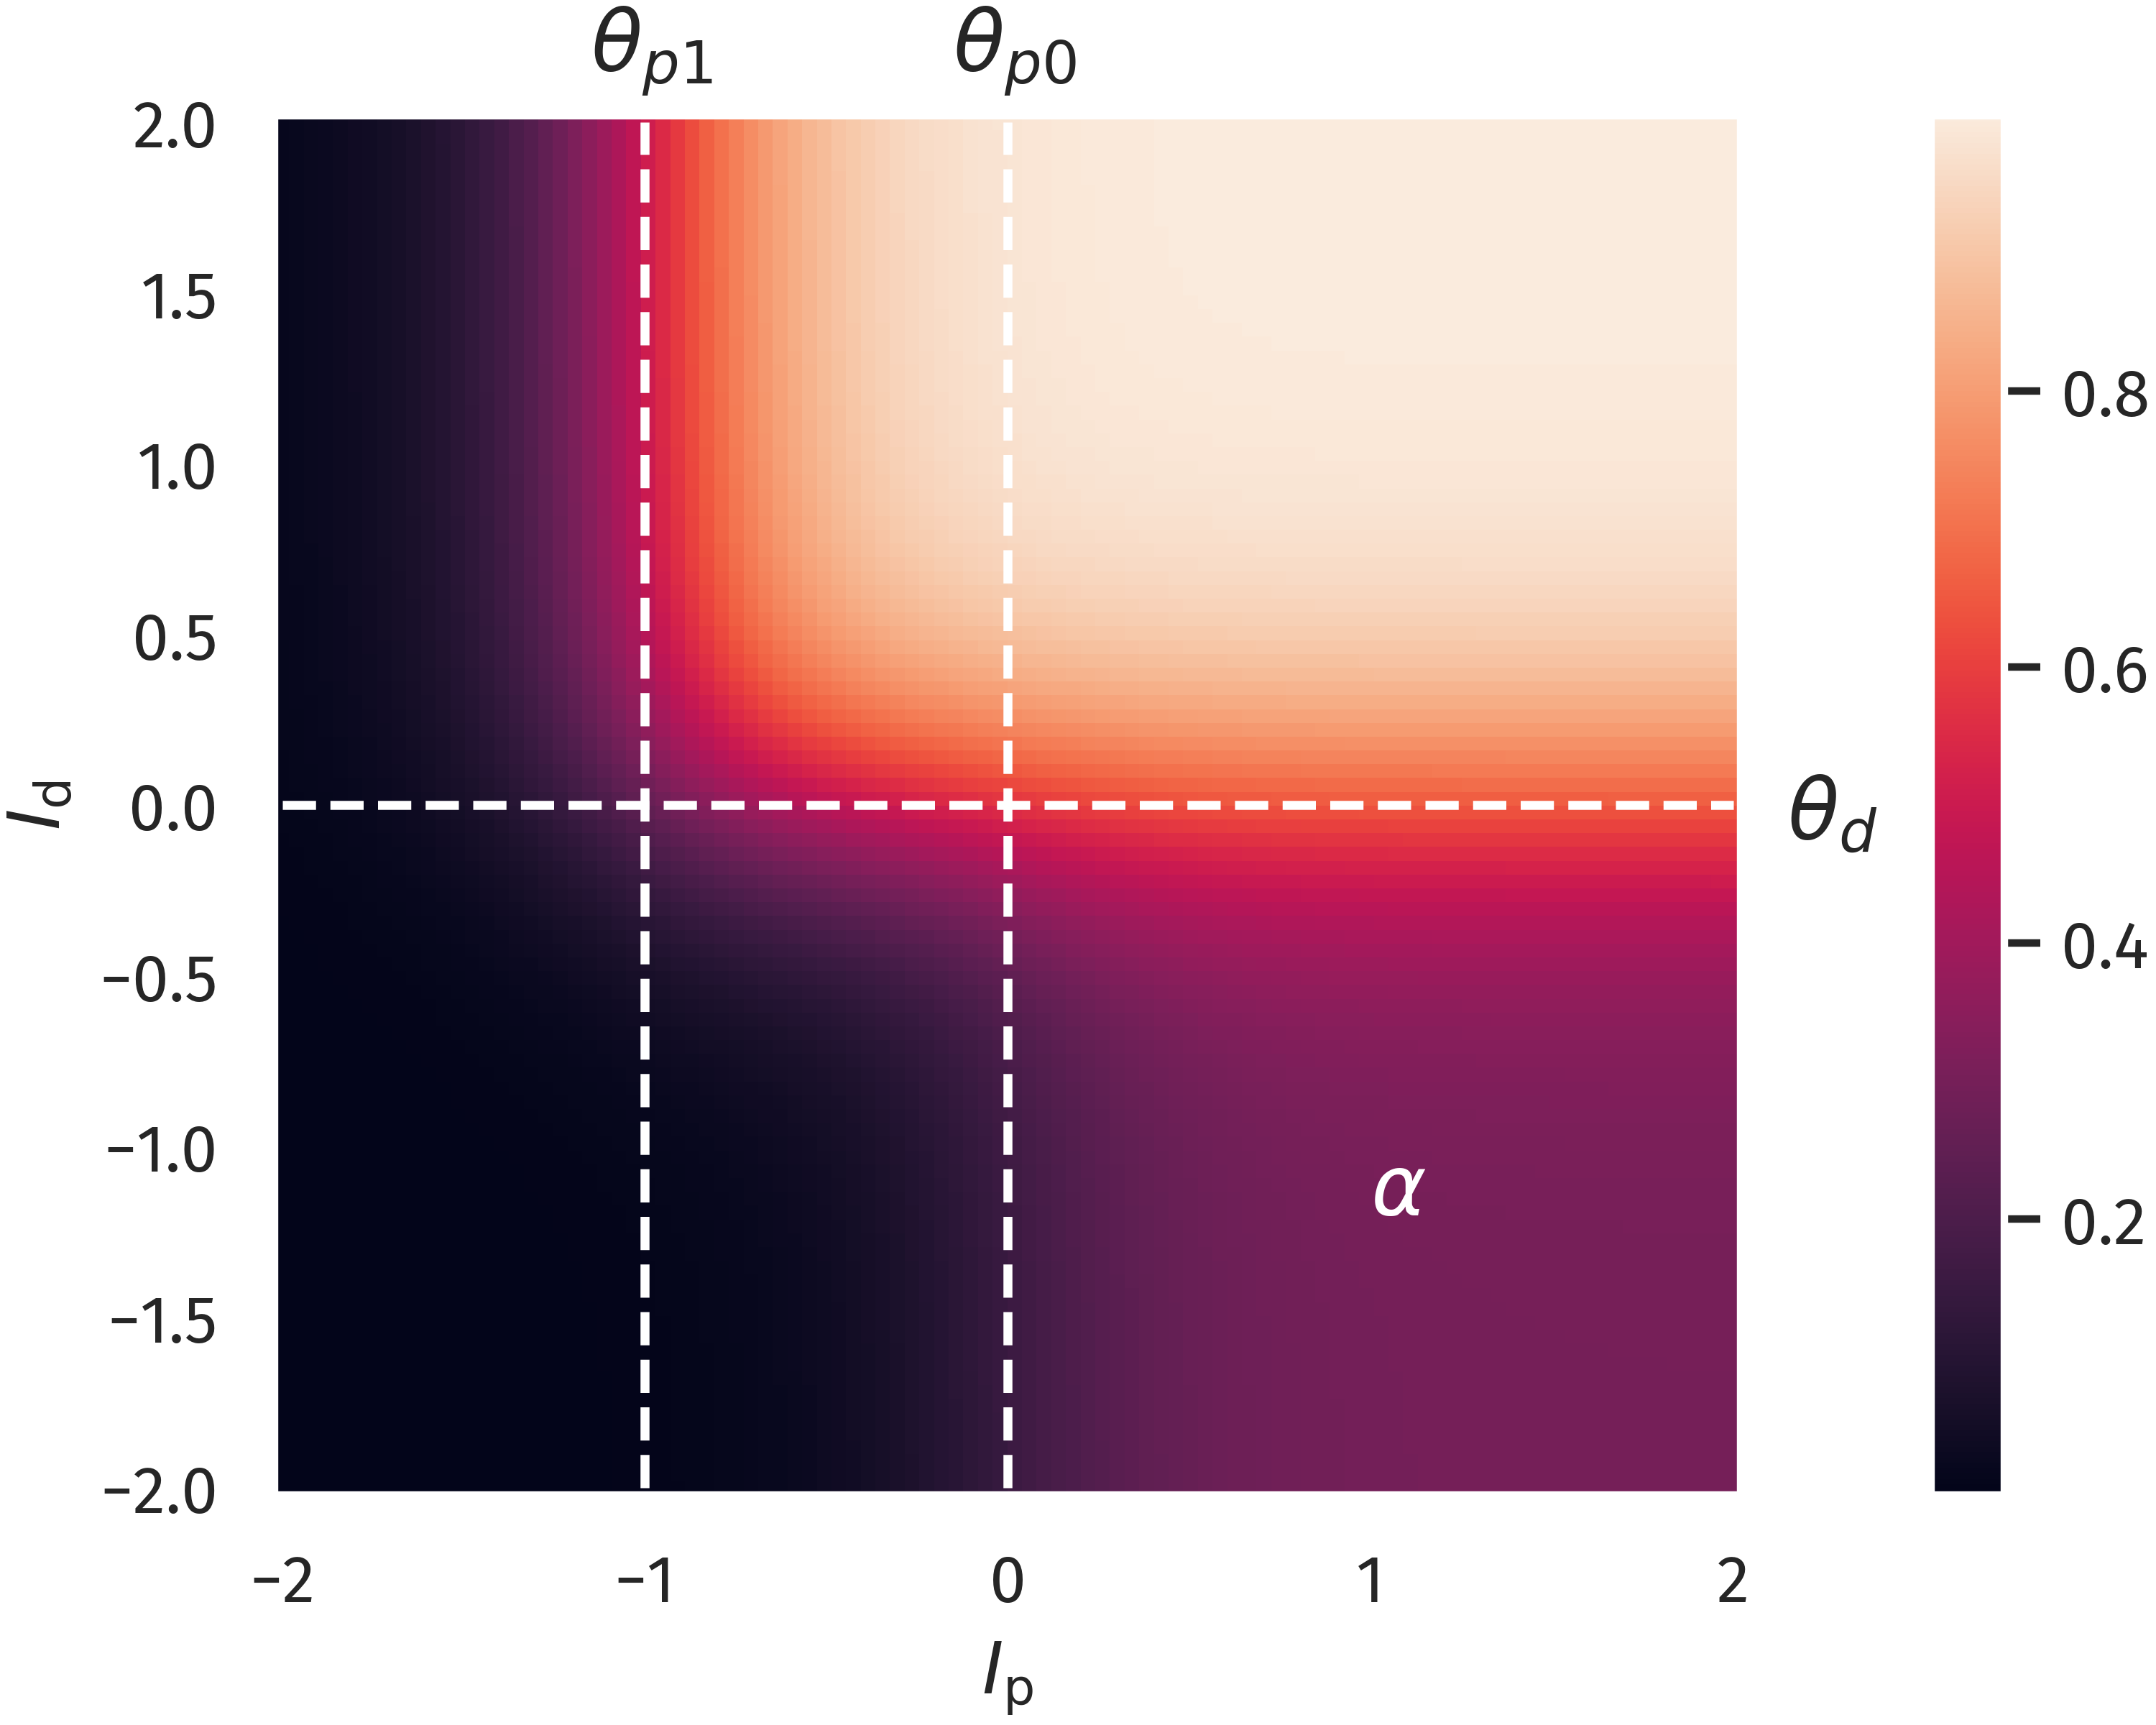
\includegraphics[width=0.6\columnwidth]{plot_comp_mod_marks.png}
\caption{{\bf Two-compartment rate model.} 
The firing rate as a function of proximal and distal 
inputs $I_p$ and $I_d$, 
see \eqref{eq_comp_model}. 
The thresholds $\theta_{p0}$, $\theta_{p1}$ and 
$\theta_d$ define two regions of neural activity,
with a a maximal firing rate of unity an a plateau
at $\alpha=0.3$.}
\label{fig:comp_model}
\end{figure}
%%%%%%%%%%%%%%%%%%%%%%%%%%%%%%%%%%%%%

In our numerical experiments we compare 
the compartment model with a classical point 
neuron, as given by
%%%%%%%%%%%%%%%%%%%%%%%%%%%%%%%%%%%%%
\begin{equation}
y(t) = \sigma\left(I_p(t) + I_d(t) - 
\theta \right) \; .
\label{eq_point_neuron}
\end{equation}
%%%%%%%%%%%%%%%%%%%%%%%%%%%%%%%%%%%%%
The apical input $I_d$ is generated
`as is', meaning, it is not dynamically 
calculated as a superposition of multiple 
presynaptic inputs. To be concrete, we
used
%%%%%%%%%%%%%%%%%%%%%%%%%%%%%%%%%%%%%
\begin{equation}
I_d(t) = n_d(t) x_d(t) - b_d(t) \; ,
\label{eq_I_d}
\end{equation}
%%%%%%%%%%%%%%%%%%%%%%%%%%%%%%%%%%%%%
where $n_d(t)$ is a scaling factor, $x_d(t)$ 
a pre-generated discrete time sequence and 
$b_d(t)$ a bias. Note that $n_d$ and $b_d$ 
are time dependent since they are subject 
to adaptation processes, which will be
described in the next section. Similarly, 
the proximal input $I_p(t)$ is given by
%%%%%%%%%%%%%%%%%%%%%%%%%%%%%%%%%%%%%
\begin{equation}
I_p(t) = n_p(t) \sum_{i=1}^{N} 
x_{p,i}(t) w_i(t) - b_p(t) \; ,
\label{eq_I_p}
\end{equation}
%%%%%%%%%%%%%%%%%%%%%%%%%%%%%%%%%%%%%
where $N$ is the number of presynaptic afferents, 
$x_{p,i}(t)$ the corresponding sequences, 
$w_i(t)$ the synaptic efficacies and
$n_p(t)$ and $b_p(t)$ the (time dependent)
scaling and bias. Tyical values for the 
parameters used throughout this study
are presented Table~\ref{tab_parameters}.

%%%%%%%%%%%%%%%%%%%%%%%%%%%%%%%%%%%%%
\begin{table}[b]
\caption{Model parameters,
as defined in sections \ref{sect:neuronmodel} and
\ref{sect_plasticity}.}
\begin{tabular}{ l | l || l | l }
		$\theta_{p0}$ & $0$ & $V_d^t$ & $0.25$ \\
		$\theta_{p1}$ & $-1$ & $\mu_b$ & $10^{-3}$ \\ 
		$\theta_{d}$ & $0$ & $\mu_n$ & $10^{-4}$ \\  
		$\alpha$ & $0.3$ & $\mu_{\rm av}$ & $5 \cdot 10^{-3}$ \\   
		$\mu_w$ & $5 \cdot 10^{-5}\quad$ & $I_p^t$ & $0$ \\
		$V_p^t$ & $0.25$ & $I_d^t$ & $0$  
\end{tabular}
\label{tab_parameters}
\end{table}
%%%%%%%%%%%%%%%%%%%%%%%%%%%%%%%%%%%%%

%---------------------------------------%
\subsection{Plasticity\label{sect_plasticity}}
%---------------------------------------%

We implemented a Hebbian plasticity rule for 
the proximal synaptic weights by the following 
update equation:
%%%%%%%%%%%%%%%%%%%%%%%%%%%%%%%%%%%%%
\begin{align}
w_i(t+1) &= w_i(t) + \mu_w \left(x_{p,i}(t) - \tilde{x}_{p,i}(t)\right)
\left(y(t) - \tilde{y} \right)
\label{eq_hebb_plast} \\
\tilde{x}_{p,i}(t+1) &= 
(1-\mu_{\rm av})\tilde{x}_{p,i}(t) + \mu_{\rm av}x_{p,i}(t) 
\label{eq_tilde_x_p_i}\\
\tilde{y}(t+1) &= (1-\mu_{\rm av})\tilde{y}(t) + \mu_{\rm av}y(t)
\label{eq_tilde_y}
\end{align}
%%%%%%%%%%%%%%%%%%%%%%%%%%%%%%%%%%%%%
The trailing time averages $\tilde{x}_{p,i}$ and
$\tilde{y}$, respectively of the presynaptic 
basal activites, $x_{p,i}$, and of the neural
firing rate $y$, enter the Hebbian learing
rule (\ref{eq_hebb_plast}) as reference levels.
Pre- and post-synaptic neurons are considered
to be active/inactive when being above/below
the respective trailing averages. The
timescale of the averaging, $1/\mu_{\rm av}$,
is typcially over 200 time steps, see
Table~\ref{tab_parameters}. 
With $1/\mu_w=2\cdot10^4$ learning is 
assumed to be be considerably slower, 
as usual for statistical update rules.
Additionally, 
we use a synaptic normalization constraint,
%%%%%%%%%%%%%%%%%%%%%%%%%%%%%%%%%%%%%
\begin{equation}
w_i(t) \rightarrow \frac{w_i(t)}{\lVert 
\mathbf{w}(t)\rVert}\;,
\label{eq:weight_norm}
\end{equation}
%%%%%%%%%%%%%%%%%%%%%%%%%%%%%%%%%%%%%
in each time step, where 
$\lVert \mathbf{w}(t)\rVert$ denotes the Euclidean
norm of the synaptic weight vector. For comparative 
reasons, the point neuron model is equipped with the
same plasticity rule for the proximal weights as 
(\ref{eq_hebb_plast}). 

The bias variables entering the definitions
\eqref{eq_I_d} and \eqref{eq_I_p} of the distal
proximal currrent, $I_d$ and $I_p$, 
are assumed to adapt accodingly to
%%%%%%%%%%%%%%%%%%%%%%%%%%%%%%%%%%%%%
\begin{align}
\label{eq_b_p_dot}
b_p(t+1) &= b_p(t) + \mu_b \left[I_p(t) - I_p^t\right] \\
b_d(t+1) &= b_d(t) + \mu_b \left[I_d(t) - I_d^t\right] \;,
\label{eq_b_d_dot}
\end{align}
%%%%%%%%%%%%%%%%%%%%%%%%%%%%%%%%%%%%%
where $I_p^t=0$ and, $I_d^t=0$
are preset targets and $1/\mu_b=10^3$ the
timescale for the adaption process. Over
time, both the distal and the proximal 
currents, $I_d$ and $I_p$, average out.

Adaption rules for the bias entering a 
transfer function, such as
\eqref{eq_b_d_dot} and \eqref{eq_b_p_dot},
have the task to regulate overall activitiy
levels. The overall magnitude of the
synaptic weights, which are determined by 
synaptic rescaling factors, here $n_d$ and $n_p$, 
as defined in \eqref{eq_I_d} and \eqref{eq_I_p},
will regulate in contrast the variance of
the neural activity, and not the average
level \citep{schubert2021local}. In this
spirit we consider
%%%%%%%%%%%%%%%%%%%%%%%%%%%%%%%%%%%%%
\begin{align}
n_d(t+1) &= n_d(t) + 
\mu_n \left[V_d^t - \left( I_d(t) - \tilde{I}_d(t)\right)^2\right] \\
n_p(t+1) &= n_p(t) + 
\mu_n \left[V_p^t - \left( I_p(t) - \tilde{I}_p(t)\right)^2\right] \\
\tilde{I}_d(t+1) &= (1-\mu_{\rm av})\tilde{I}_d(t) + \mu_{\rm av} I_d(t) \\
\tilde{I}_p(t+1) &= (1-\mu_{\rm av})\tilde{I}_p(t) + \mu_{\rm av} I_p(t) 
\end{align}
%%%%%%%%%%%%%%%%%%%%%%%%%%%%%%%%%%%%%
Here, $V_p^t$ and $V_p^t$ define targets for 
the temporal averaged variances of $I_p$ 
and $I_d$.  
The dynamic variables $\tilde{I}_p$ and $\tilde{I}_d$ 
are simply low-pass filtered running averages of 
$I_p$ and $I_d$. Overall, the framework
specified here allows the neuron to be fully flexible,
as long as the activtiy level and its variance 
fluctuate around preset target values 
\citep{schubert2021local}. A list of 
the parameter values used throughout this investigation 
is given in Table~\ref{tab_parameters}. Our choices of
target means and variances are based on the assumption
that neural input should be tuned towards a certain
working regime of the neural transfer function. In
the case of the presented model, this means that both
proximal and distal input cover an area where the nonlinearities
of the transfer function are reflected without oversaturation.

%%%%%%%%%%%%%%%%%%%%%%%%%%%%%%%%%%%%%
\begin{figure}[t]
\centering
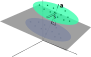
\includegraphics[width=0.55\columnwidth]{illustration_classification}
\caption{{\bf Input Space for the Linear Classification Task.}
Two clusters of presynaptic basal activities were generated from 
multivariate Gaussian distributions. Here, $s$ denotes the standard
deviation orthogonal to the normal vector $\mathbf{a}$ of the 
classification hyperplane, as defined by \eqref{eq_x_d_a}.}
\label{fig_illustration_classification}
\end{figure}
%%%%%%%%%%%%%%%%%%%%%%%%%%%%%%%%%%%%%

%---------------------------------------%
\section{Results}
\label{sect:results}
%---------------------------------------%

%---------------------------------------%
\subsection{Unsupervised Alignment between Basal and Apical Inputs}
\label{sect:alignment}
%---------------------------------------%

As a first test, we quantify the neuron's ability to 
align its basal input to the apical teaching signal.
This can be done using the pearson correlation coefficient
$\rho[I_p,I_d]$ between the basal and 
apical input currents. We determined 
$\rho[I_p,I_d]$ after the simulation,
which involves all plasticity mechanisms, both
for the synaptic weights and for the intrinsic 
parameters. The input sequences $x_{p,i}(t)$ 
is randomly drawn from a uniform distribution,
in $[0,1]$, which is done independently for 
each $i\in[1,N]$.

For the distal current $I_d(t)$ to be fully 
`reconstructable' by the basal input, $x_d(t)$ has 
to be a linear combination 
%%%%%%%%%%%%%%%%%%%%%%%%%%%%%%%%%%%%%
\begin{align}
x_d(t) &= \sum_{i=1}^N a_i x_{p,i}(t)
\label{eq_x_d_a}
\end{align}
%%%%%%%%%%%%%%%%%%%%%%%%%%%%%%%%%%%%%
of the $x_{p,i}(t)$, where the $a_i$ are the
components of a random vector $\mathbf{a}$ 
of unit length. 

Given that we use with \eqref{eq_hebb_plast}
a Hebbian learning scheme, one can expect that
the direction and the magnitude of the principal 
components of the basal input may affect the
outcome of the simulation significantly:
A large variance in the basal input 
orthogonal to the `reconstruction vector' $\mathbf{a}$ 
is a distraction for the plasticity. The
observed temporal alignment between $I_p$ and 
$I_d$ should hence suffer when such a 
distraction is present. The situaton is illustrated 
in Fig.~\ref{fig_illustration_classification}.

In order to test the effects of distracting directions,
we applied a transformation to the input sequences $x_{p,i}(t)$.
For the transformation two parameters are used,
a scaling factor $s$ and the dimension $N_{\rm dist}$ 
of the distracting subspace within the basal input 
space. The $N_{\rm dist}$ randomly generated
basis vectors are orthogonal to the superposition
vector $\mathbf{a}$, as defined by \eqref{eq_x_d_a},
and to each others. Within this $N_{\rm dist}$-dimensional 
subspace, the input sequences $x_{p,i}(t)$ are
rescaled subsequently by the factor $s$. 
See Fig.~\ref{fig_illustration_classification}.
After the learning phase, a second set of input 
sequences $x_{p,i}(t)$ and $x_d(t)$ is generated for 
testing purposes, using the identical protocol, and
the cross correlation $\rho[I_p,I_d]$ 
evaluated. During the testing phase plasticity is 
turned off.

%%%%%%%%%%%%%%%%%%%%%%%%%%%%%%%%%%%%%
\begin{figure}[t]
\centering
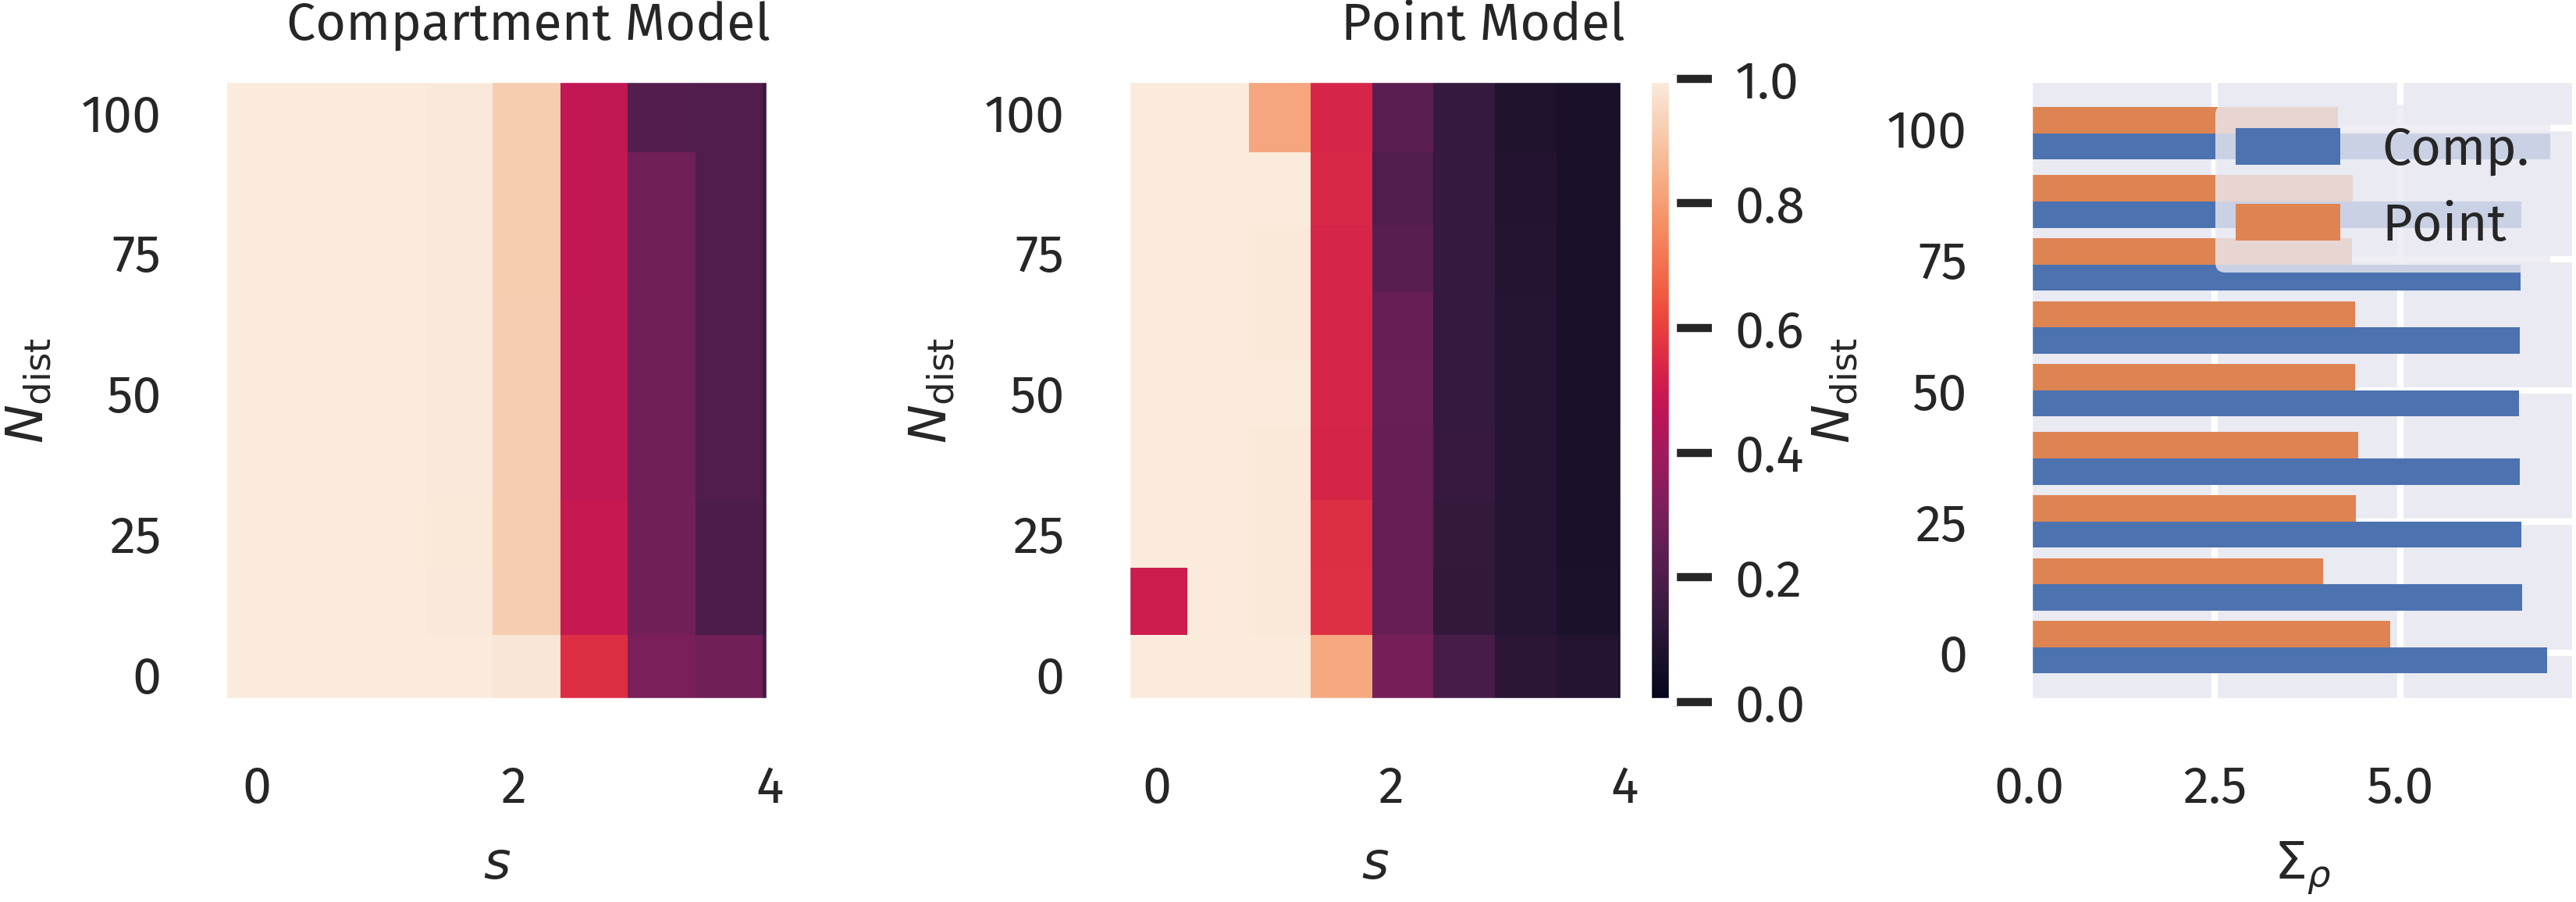
\includegraphics[width=1.0\columnwidth]{corr_dimension_scaling_high_input_dim}
\caption{{\bf Unsupervised Alignment between 
Basal and Apical Input.} Color
encoded the Pearson correlation $\rho[I_p,I_d]$ 
between the proximal and distal input currents,
$I_p$ and $I_d$. Data for a range of the orthogonal 
distraction directions, $N_{\rm dist}\in[0,N-1]$, 
and the scaling factor $s$, as defined in
Fig.~\ref{fig_illustration_classification}.
The overall number of basal inputs is $N=100$.
The quantity $\Sigma_{\rho}$ depicted in the bar
plot is the sum, for a given $N_{\rm dist}$,
over the correlation values $s=0,\,0.5,\,1.0\,..$ 
used for the simulation run. Blue bars represents 
the compartment model, orange the point model.}
%\Delta s = 10/(N_s-1) von 0 bis 10.
% > D.h.  s\in[0,10],   N_s = 20 ?
\label{fig_corr_dimension_scaling}
\end{figure}
%%%%%%%%%%%%%%%%%%%%%%%%%%%%%%%%%%%%%

The overall aim of our portocal is to evaluate
the degree $\rho[I_p,I_d]$ to which
the proximal current $I_p$ aligns in the
temporal domain to the distal input $I_d$.
We recall that this is a highly non-trivial
question, given that the proximal synpatic
weights are adapted via Hebbian plasticity, 
see \eqref{eq_hebb_plast}. The error 
$(I_p-I_d)^2$ does not
enter the adaption rules employed.
Results are presented in
Fig.~\ref{fig_corr_dimension_scaling}
as a function of the distraction parameters 
$s$ and $N_{\rm dist}\in[0,N-1]$. The
total number of basal inputs is $N=100$.

For a comparison, in 
Fig.~\ref{fig_corr_dimension_scaling}
data for both the compartment model
and for a point neuron are presented,
as defined respectively by \eqref{eq_comp_model}
and \eqref{eq_point_neuron}. A decorrelation 
transition as a function of the distraction 
scaling paramerer $s$ is observed for both 
models. However, the compartment model is able
to handle a significantly stronger distraction 
as compared to the point model. These findings
support the hypothesis examined here, namely
that nonlinear interactions between basal and 
apical input improve learning guided by top-down signals.

%---------------------------------------%
\subsection{Supervised Learning in a Linear Classification Task}
\label{sect:classification}
%---------------------------------------%

Next, we investigated if the observed differences would also improve
the performance in an actual supervised learning task.
For this purpose, we constructed presynaptic basal 
input $x_p(t)$ as illustrated in 
Fig.~\ref{fig_illustration_classification}.
Written in vector form, each sample from the basal 
input is generated from the following expression:
%%%%%%%%%%%%%%%%%%%%%%%%%%%%%%%%%%%%%
\begin{equation}
\mathbf{x}_p(t) = \mathbf{b} + \mathbf{a}\left(c(t) + \sigma_a \zeta_a(t) \right) 
+ s \cdot \sum_{i=1}^{N_{\rm dist}} \zeta_{dist,i}(t) \mathbf{v}_{dist,i} \; .
\end{equation}
%%%%%%%%%%%%%%%%%%%%%%%%%%%%%%%%%%%%%
Here, $\mathbf{b}$ is a random vector drawn uniformly from
$(0,1)^N$, $\mathbf{a}$ is random unit vector as introduced in 
Section~\ref{sect:alignment}, $c(t)$ is a binary variable drawn 
from $\{-0.5,0.5\}$ with equal probability and $\zeta_a(t)$ and the
$\zeta_{dist,i}(t)$ are independent random Gaussian variables with 
zero mean and unit variance. 
Hence, $\sigma_a$ simply denotes the standard deviation of each Gaussian
cluster along the direction of the normal vector $\mathbf{a}$ and was
set to $\sigma_a = 0.25$. 
Finally, the set of $\mathbf{v}_{dist,i}$ forms a randomly generated
orthogonal basis of $N_{\rm dist}$ unit vectors which---just as in 
Section~\ref{sect:alignment}---are also orthogonal to $\mathbf{a}$.
The free parameter $s$ parameterized
the standard deviation along this subspace orthogonal to $\mathbf{a}$.
As indicated by the time dependence, the Gaussian and binary random
variables are drawn for each time step. The vectors
$\mathbf{b}$, $\mathbf{a}$, and $\mathbf{v}_{dist,i}$ are generated
once before the beginning of a simulation run.

For the classification task, we set up two output neurons receiving
the same basal presynaptic input, while the top-down input encoded
the correct linear classification in a one-hot scheme, that is
%%%%%%%%%%%%%%%%%%%%%%%%%%%%%%%%%%%%%
\begin{align}
x_{d,0}(t) &= 1 - \Theta\left( \left(\mathbf{x}_p(t) - 
\mathbf{b}\right)^T \mathbf{a}\right) \\
x_{d,1}(t) &= \Theta\left( \left(\mathbf{x}_p(t) - 
\mathbf{b}\right)^T \mathbf{a}\right) \; ,
\end{align}
%%%%%%%%%%%%%%%%%%%%%%%%%%%%%%%%%%%%%
where $\Theta(x)$ is the Heaviside step function.

As in the previous experiment, we ran a full simulation until 
all dynamic variables reached a stationary state. After this,
a test run without plasticity and with the apical input turned off 
was used to evaluate the classification	performance. 
For each sample, the index of the neuron with the highest 
activity was used as the predicted class. 
Accuracy was then calculated as the fraction
of correctly classified samples.
%%%%%%%%%%%%%%%%%%%%%%%%%%%%%%%%%%%%%
\begin{figure}[t]
\centering
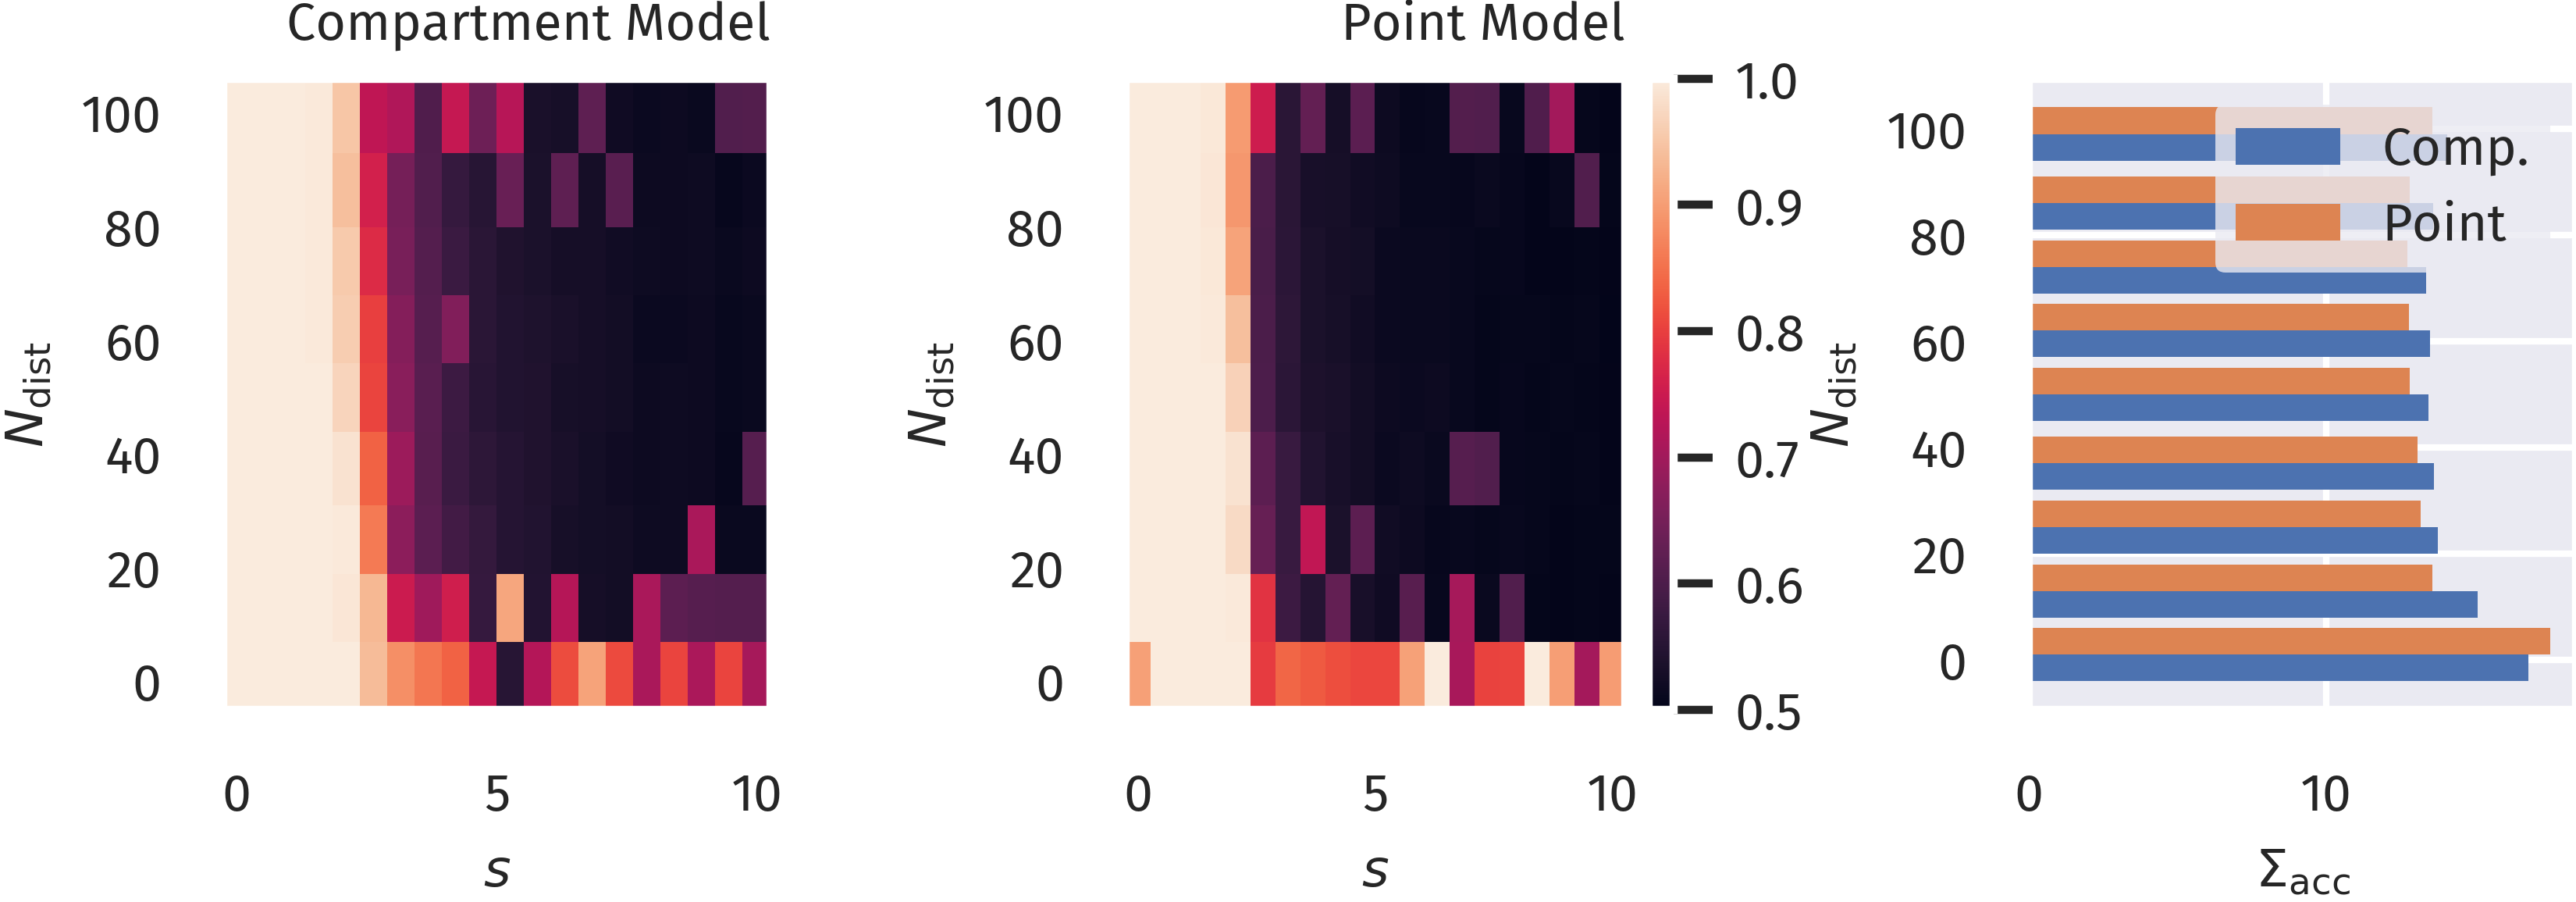
\includegraphics[width=1.0\columnwidth]{classification_dimension_scaling_high_input_dim}
\caption{{\bf Binary Classification Accuracy.}
	Fraction of correctly classified patterns as illustrated in
	Fig.~\ref{fig_illustration_classification}, see 
	Section~\ref{sect:classification}. The quantity $\Sigma_{\rm acc}$ depicted in the bar
	plot is the sum over all accuracies for the different tested values
	of $s$ under a given $N_{\rm dist}$. Blue bar represents the compartment model,
	orange the point model.}
\label{fig:classification_accuracy}
\end{figure}
%%%%%%%%%%%%%%%%%%%%%%%%%%%%%%%%%%%%%

The resulting accuracy as a function of $N_{\rm dist}$ and $s$
is shown in Fig.~\ref{fig:classification_accuracy}.
Albeit differences are small, the compartment model does
show a better overall accuracy for the tested parameter range.
It should be noted, though, that the advantage of the compartment
model becomes even less prominent when looking at the actual
correlation between proximal and distal input as a
measure of successful learning (as done in the previous section).
Fig.~\ref{fig:classification_correlation} in the supplementary 
section shows that the compartment model allows for a marginally
larger scaling among the distraction dimensions.
\\
%---------------------------------------%
\subsection{Generalized Hebbian Learning Rules}
\label{sect:non-hebbian}
%---------------------------------------%

Instead of basic Hebbian learning, we also considered 
a BCM-like learning rule for the basal weights 
\citep{Bienenstock1982,Intrator1992}.
The form of the BCM-rule used here reads
%%%%%%%%%%%%%%%%%%%%%%%%%%%%%%%%%%%%%
\begin{equation}
\Delta w_i \propto y\left(y - \theta_M\right) x_i - 
\epsilon w_i \; , \label{eq:bcm_rule}
\end{equation}
%%%%%%%%%%%%%%%%%%%%%%%%%%%%%%%%%%%%%
where $\theta_M$ is a threshold defining a transition from LTP to LTD and
$\epsilon$ is an optional decay term on the weights.
In the variant introduced by \citet{Law1994}, the sliding threshold is simply
the temporal average of the squared neural activity, 
$\theta_M = \langle y^2 \rangle$. In practice, this would be calculated
as a running average, thereby preventing the weights from growing 
indefinitely.

However, for our compartment model, we chose to explicitly set the
threshold to be the mean value between the high- and low-activity regime
in our compartment model, i.e.\ $\theta_M = (1+\alpha)/2$. By doing so, LTP is
preferably induced if both basal and apical input are present at the same
time. Furthermore, instead of the weight decay term, we chose to keep
the weight normalization as introduced in \eqref{eq:weight_norm}.
Obviously, for the point model, the reasoning behind our choice of
$\theta_M$ did not apply. Still, to provide some level of comparability,
we also ran simulations with a point model where the sliding threshold was
calculated as a running average of $y^2$. Furthermore, we did not use
weight normalization in this case, but chose to use a small weight decay term
with $\epsilon = 0.1$. The results are shown in 
Fig.~\ref{fig:classification_accuracy_bcm} (classification task) and 
Fig.~\ref{fig:classification_accuracy_bcm} (Basal-Apical alignment). 
While the accuracy of the classification for the point model
is at most comparable to Hebbian learning, the BCM-like rule for the 
compartment model significantly increases the accuracy for the tested
parameter range (compare Fig.~\ref{fig:classification_accuracy}). 
Still, as for the Hebbian learning rule, this result should be taken
with a grain of salt, as Fig.~\ref{fig:classification_correlation_bcm}
in the supplementary section indicates that a rather large part of 
the region ($s>5$) showing good
classification performance for the compartment model in 
Fig.~\ref{fig:classification_accuracy_bcm} does hardly exhibit any actual
correlation between proximal and distal input, making it likely that
the accuracy of the classification could be easily impaired in this regime, 
e.g.\ by injecting small amounts of noise.

The compartment model also significantly benefits from
the BCM rule in terms of basal-apical alignment as tested in 
Sect.~\ref{sect:alignment}, while only marginal
improvements can be observed for the point model
(compare Fig.~\ref{fig_corr_dimension_scaling_bcm} 
with Fig.~\ref{fig_corr_dimension_scaling}).
%%%%%%%%%%%%%%%%%%%%%%%%%%%%%%%%%%%%%
\begin{figure}[t]
\centering
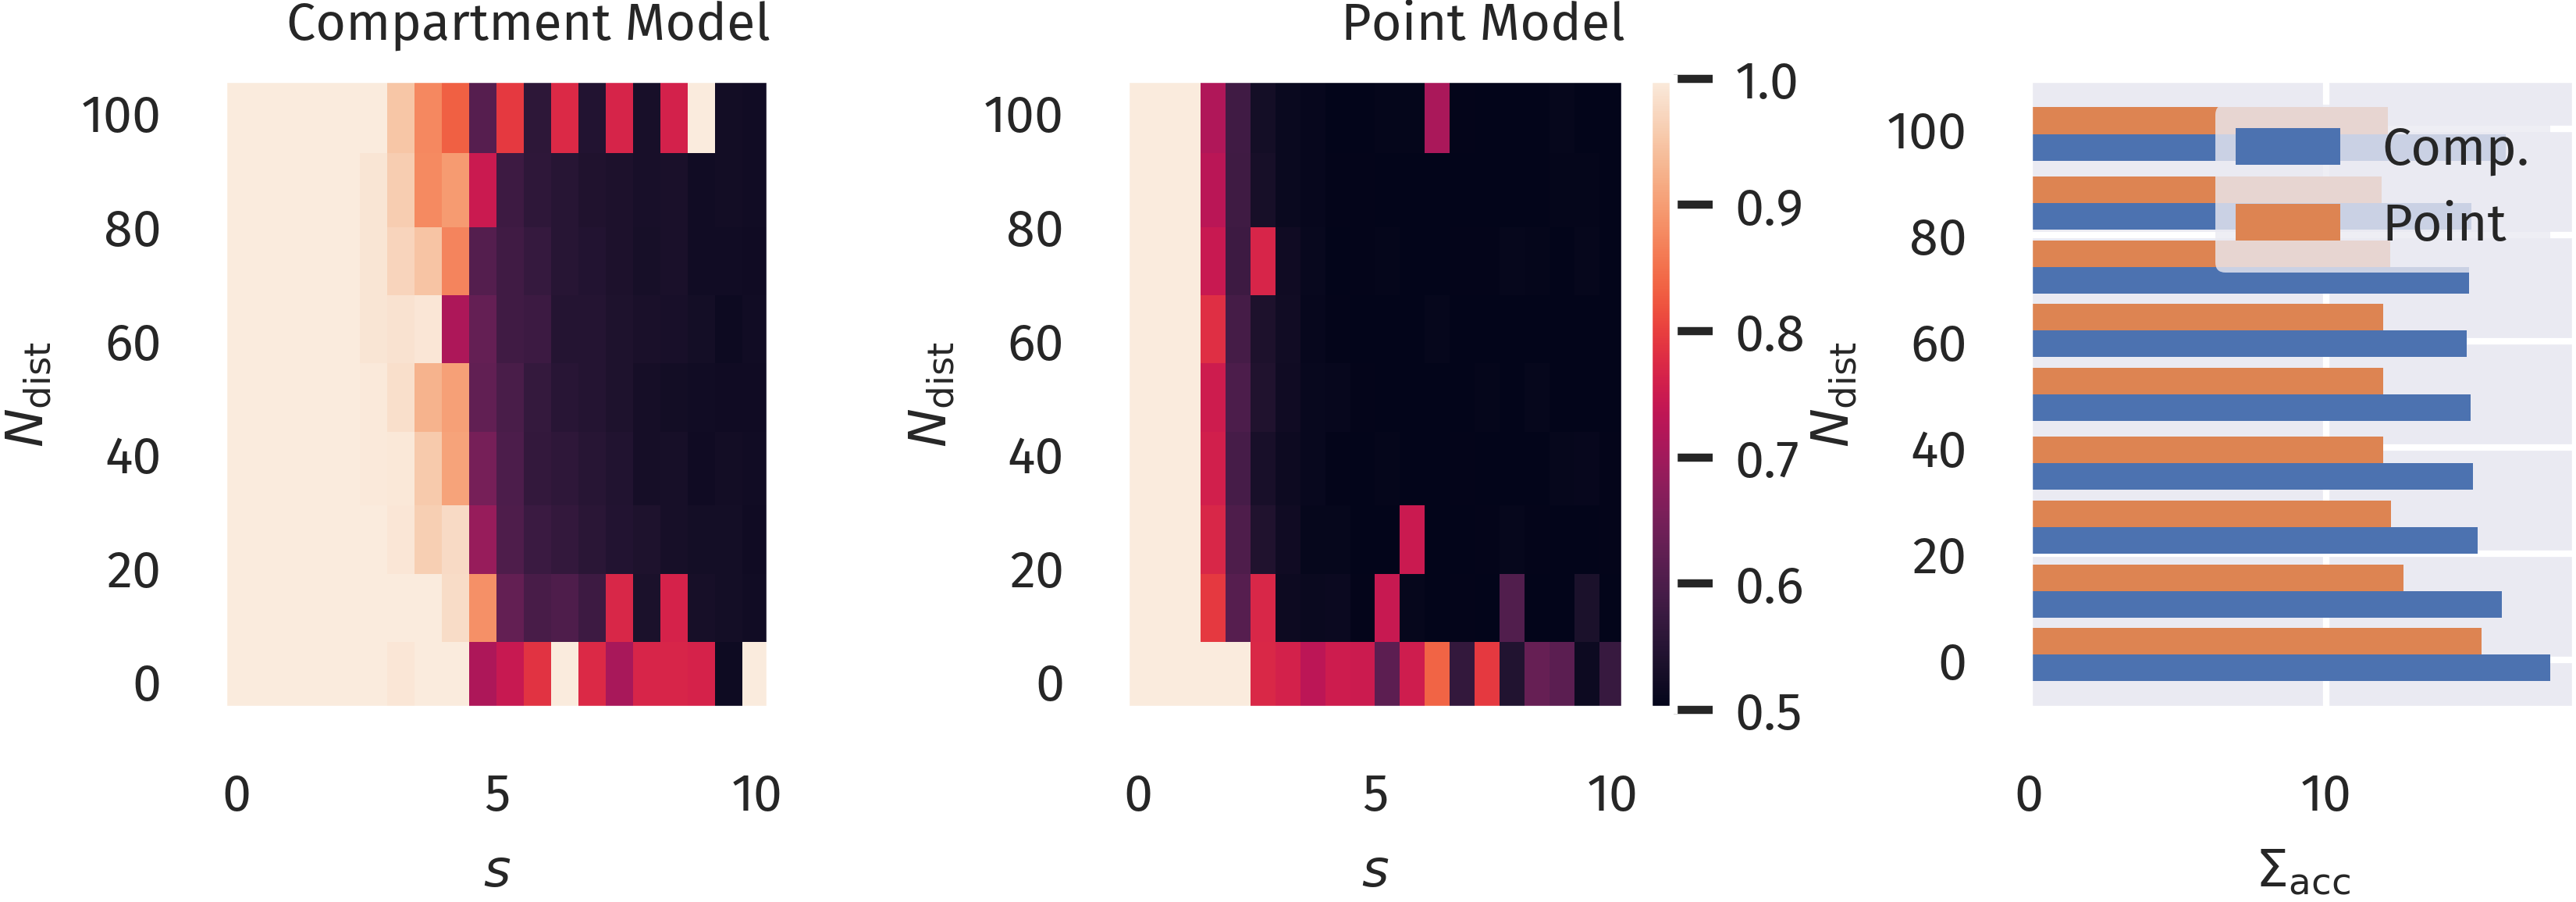
\includegraphics[width=1.0\columnwidth]{classification_dimension_scaling_bcm_high_input_dim}
\caption{{\bf Binary Classification Accuracy, BCM Rule.}
	Fraction of correctly classified patterns as illustrated in
	Fig.~\ref{fig_illustration_classification}, after training with
	a BCM-like learning rule. The quantity $\Sigma_{\rm acc}$ depicted in the bar
	plot is the sum over all accuracies for the different tested values
	of $s$ under a given $N_{\rm dist}$. Blue bar represents the compartment model,
	orange the point model.}
\label{fig:classification_accuracy_bcm}
\end{figure}
%%%%%%%%%%%%%%%%%%%%%%%%%%%%%%%%%%%%%
%%%%%%%%%%%%%%%%%%%%%%%%%%%%%%%%%%%%%
\begin{figure}[t]
\centering
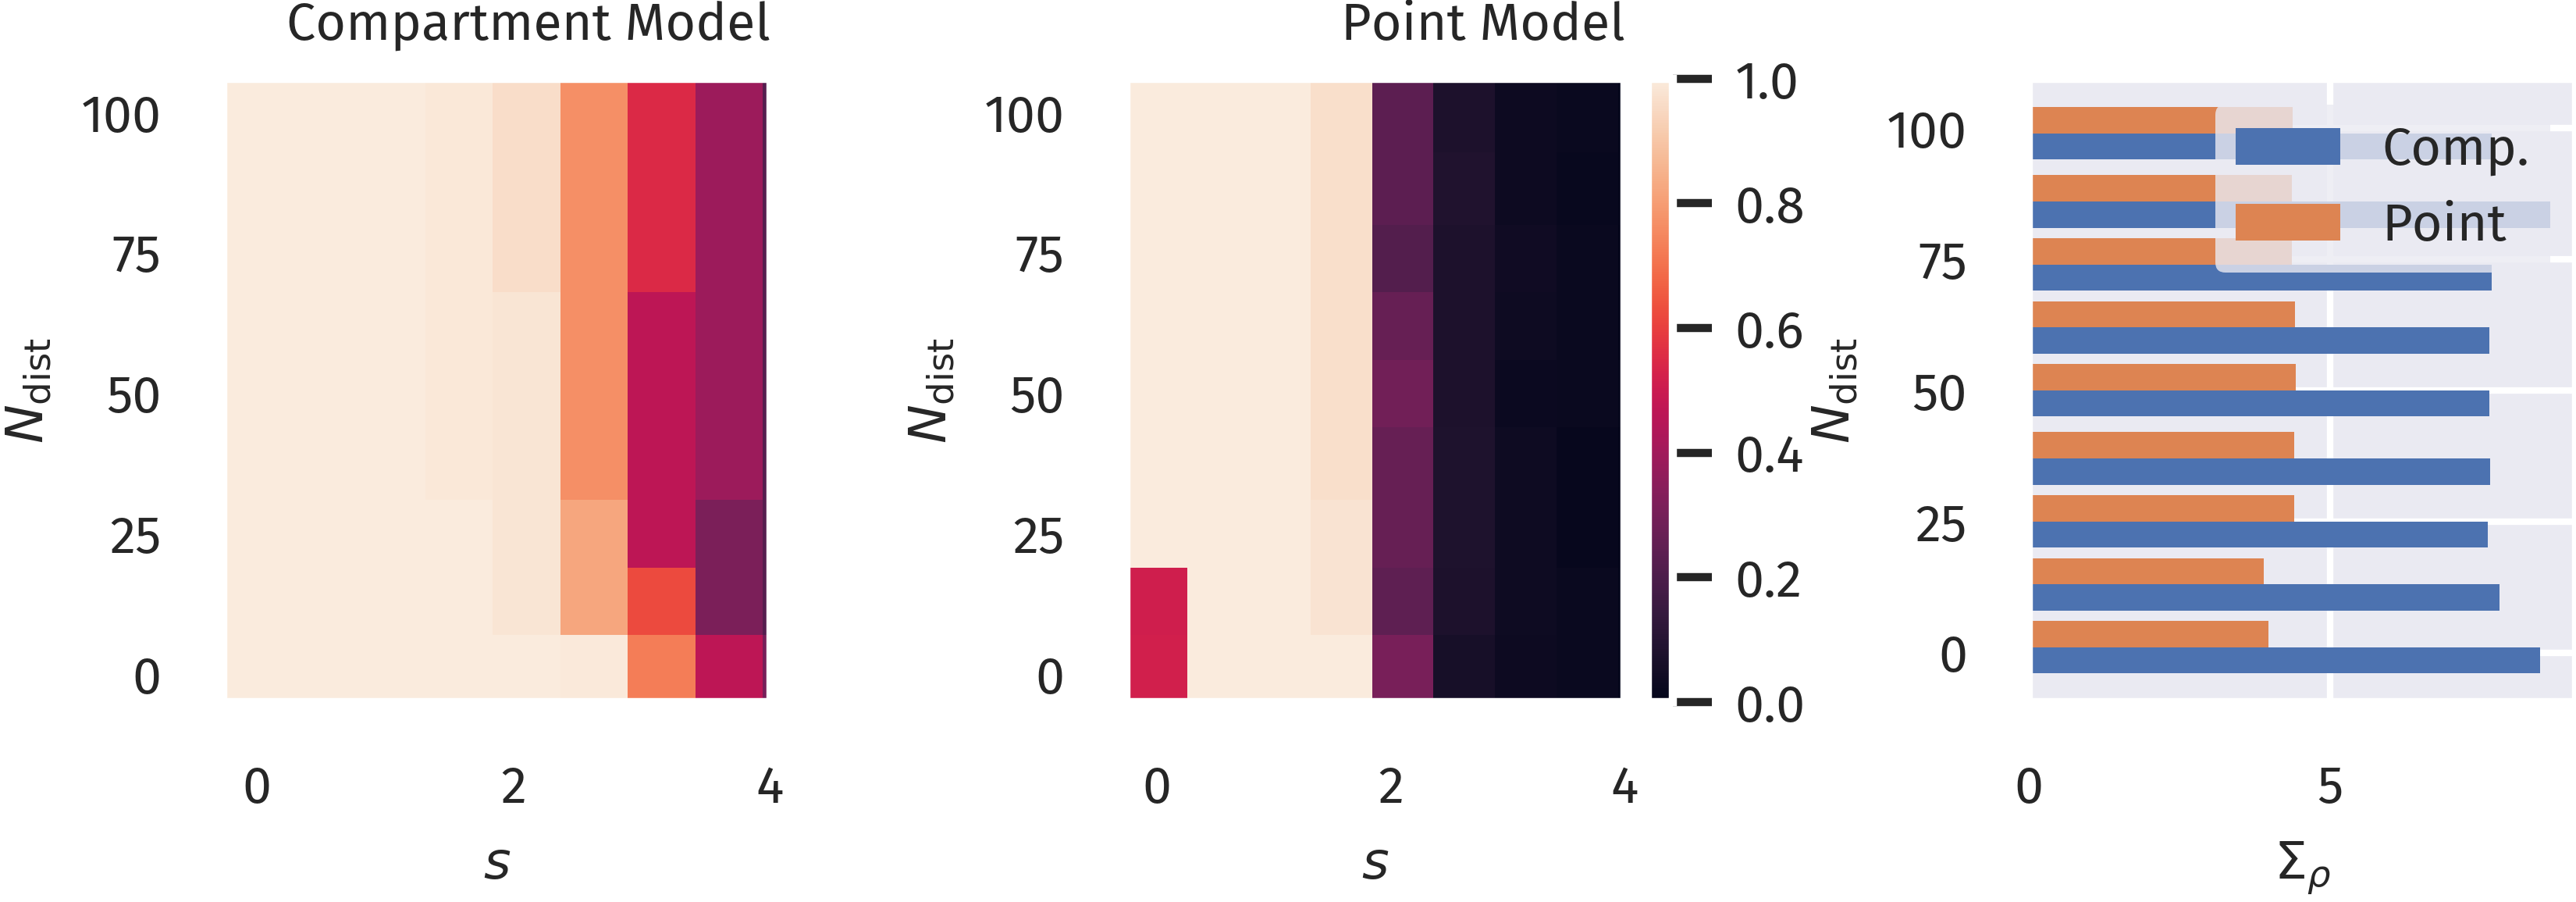
\includegraphics[width=1.0\columnwidth]{corr_dimension_scaling_bcm_high_input_dim}
\caption{{\bf Alignment between Basal and Apical Input, BCM Rule.}
Color encodes the Pearson correlation $\rho[I_p,I_d]$ for different
number of orthogonal distraction directions $N_{\rm dist}$ 
and the corresponding scaling faction $s$ after training
with a BCM-like rule. The quantity $\Sigma_{\rho}$ depicted in the bar
plot is the sum over all correlation values for the different tested values
of $s$ under a given $N_{\rm dist}$. Blue bar represents the compartment model,
orange the point model. Compare to Fig.~\ref{fig_corr_dimension_scaling}.}
\label{fig_corr_dimension_scaling_bcm}
\end{figure}
%%%%%%%%%%%%%%%%%%%%%%%%%%%%%%%%%%%%%
\\
\\
%---------------------------------------%
\subsection{Objective Function of BCM Learning in the Compartment Model}
\label{sect:Obj_Func}
%---------------------------------------%

To form a better understanding of why the BCM-type learning rule
in combination with the implemented compartment model, we can formalize
the learning rule for the proximal weights in terms of an objective function.
For this purpose, we further simplify \eqref{eq_comp_model} by replacing
the sigmoid functions $\sigma(x)$ by a simple step function $\Theta(x)$. 
This does not change the overall shape or topology of the activation
in the $(I_p,I_d)$ space but merely makes the smooth transitions sharp
and instantaneous. Using $\Delta w_i \propto y\left(y - \theta_M \right) x_i$,
we find in this case
%%%%%%%%%%%%%%%%%%%%%%%%%%%%%%%%%%%%%
\begin{equation}
\begin{split}
\Delta w_i \propto [ (1-\alpha) \Theta(I_d - \theta_{d})\Theta(p-\theta_{p1})
\\ + \alpha (\alpha - 1)\Theta(\theta_{d} - I_d)\Theta(p-\theta_{p0}) ]x_i \; .
\end{split}
\end{equation}
%%%%%%%%%%%%%%%%%%%%%%%%%%%%%%%%%%%%%
Noting that $\Theta(x)$ is the first derivative of the ReLu function $[x]^+ \equiv \max(0,x)$,
we find that this update rule can be written as
%%%%%%%%%%%%%%%%%%%%%%%%%%%%%%%%%%%%%
\begin{align}
\Delta w_i &\propto \frac{\partial \mathcal{L}_p}{\partial w_i}\\
\begin{split}
\mathcal{L}_p &\equiv (1-\alpha) \Theta(I_d - \theta_{d})[p-\theta_{p1}]^+\\
&\;\; + \alpha (\alpha - 1)\Theta(\theta_{d} - I_d)[p-\theta_{p0}]^+ \; .
\end{split}\label{eq:obj_func}
\end{align}
%%%%%%%%%%%%%%%%%%%%%%%%%%%%%%%%%%%%%
The objective function is shown in Fig.~\ref{fig:obj_func}. 
One can observe that states closer to the $I_p$-$I_d$ diagonal 
are preferred, while the opposite is the case for off-diagonal states. 
This provides an explanation why the BCM-rule can induce 
an alignment between proximal and distal inputs when used 
in combination with the nonlinear compartment model. 
%%%%%%%%%%%%%%%%%%%%%%%%%%%%%%%%%%%%%
\begin{figure}[t]
\centering
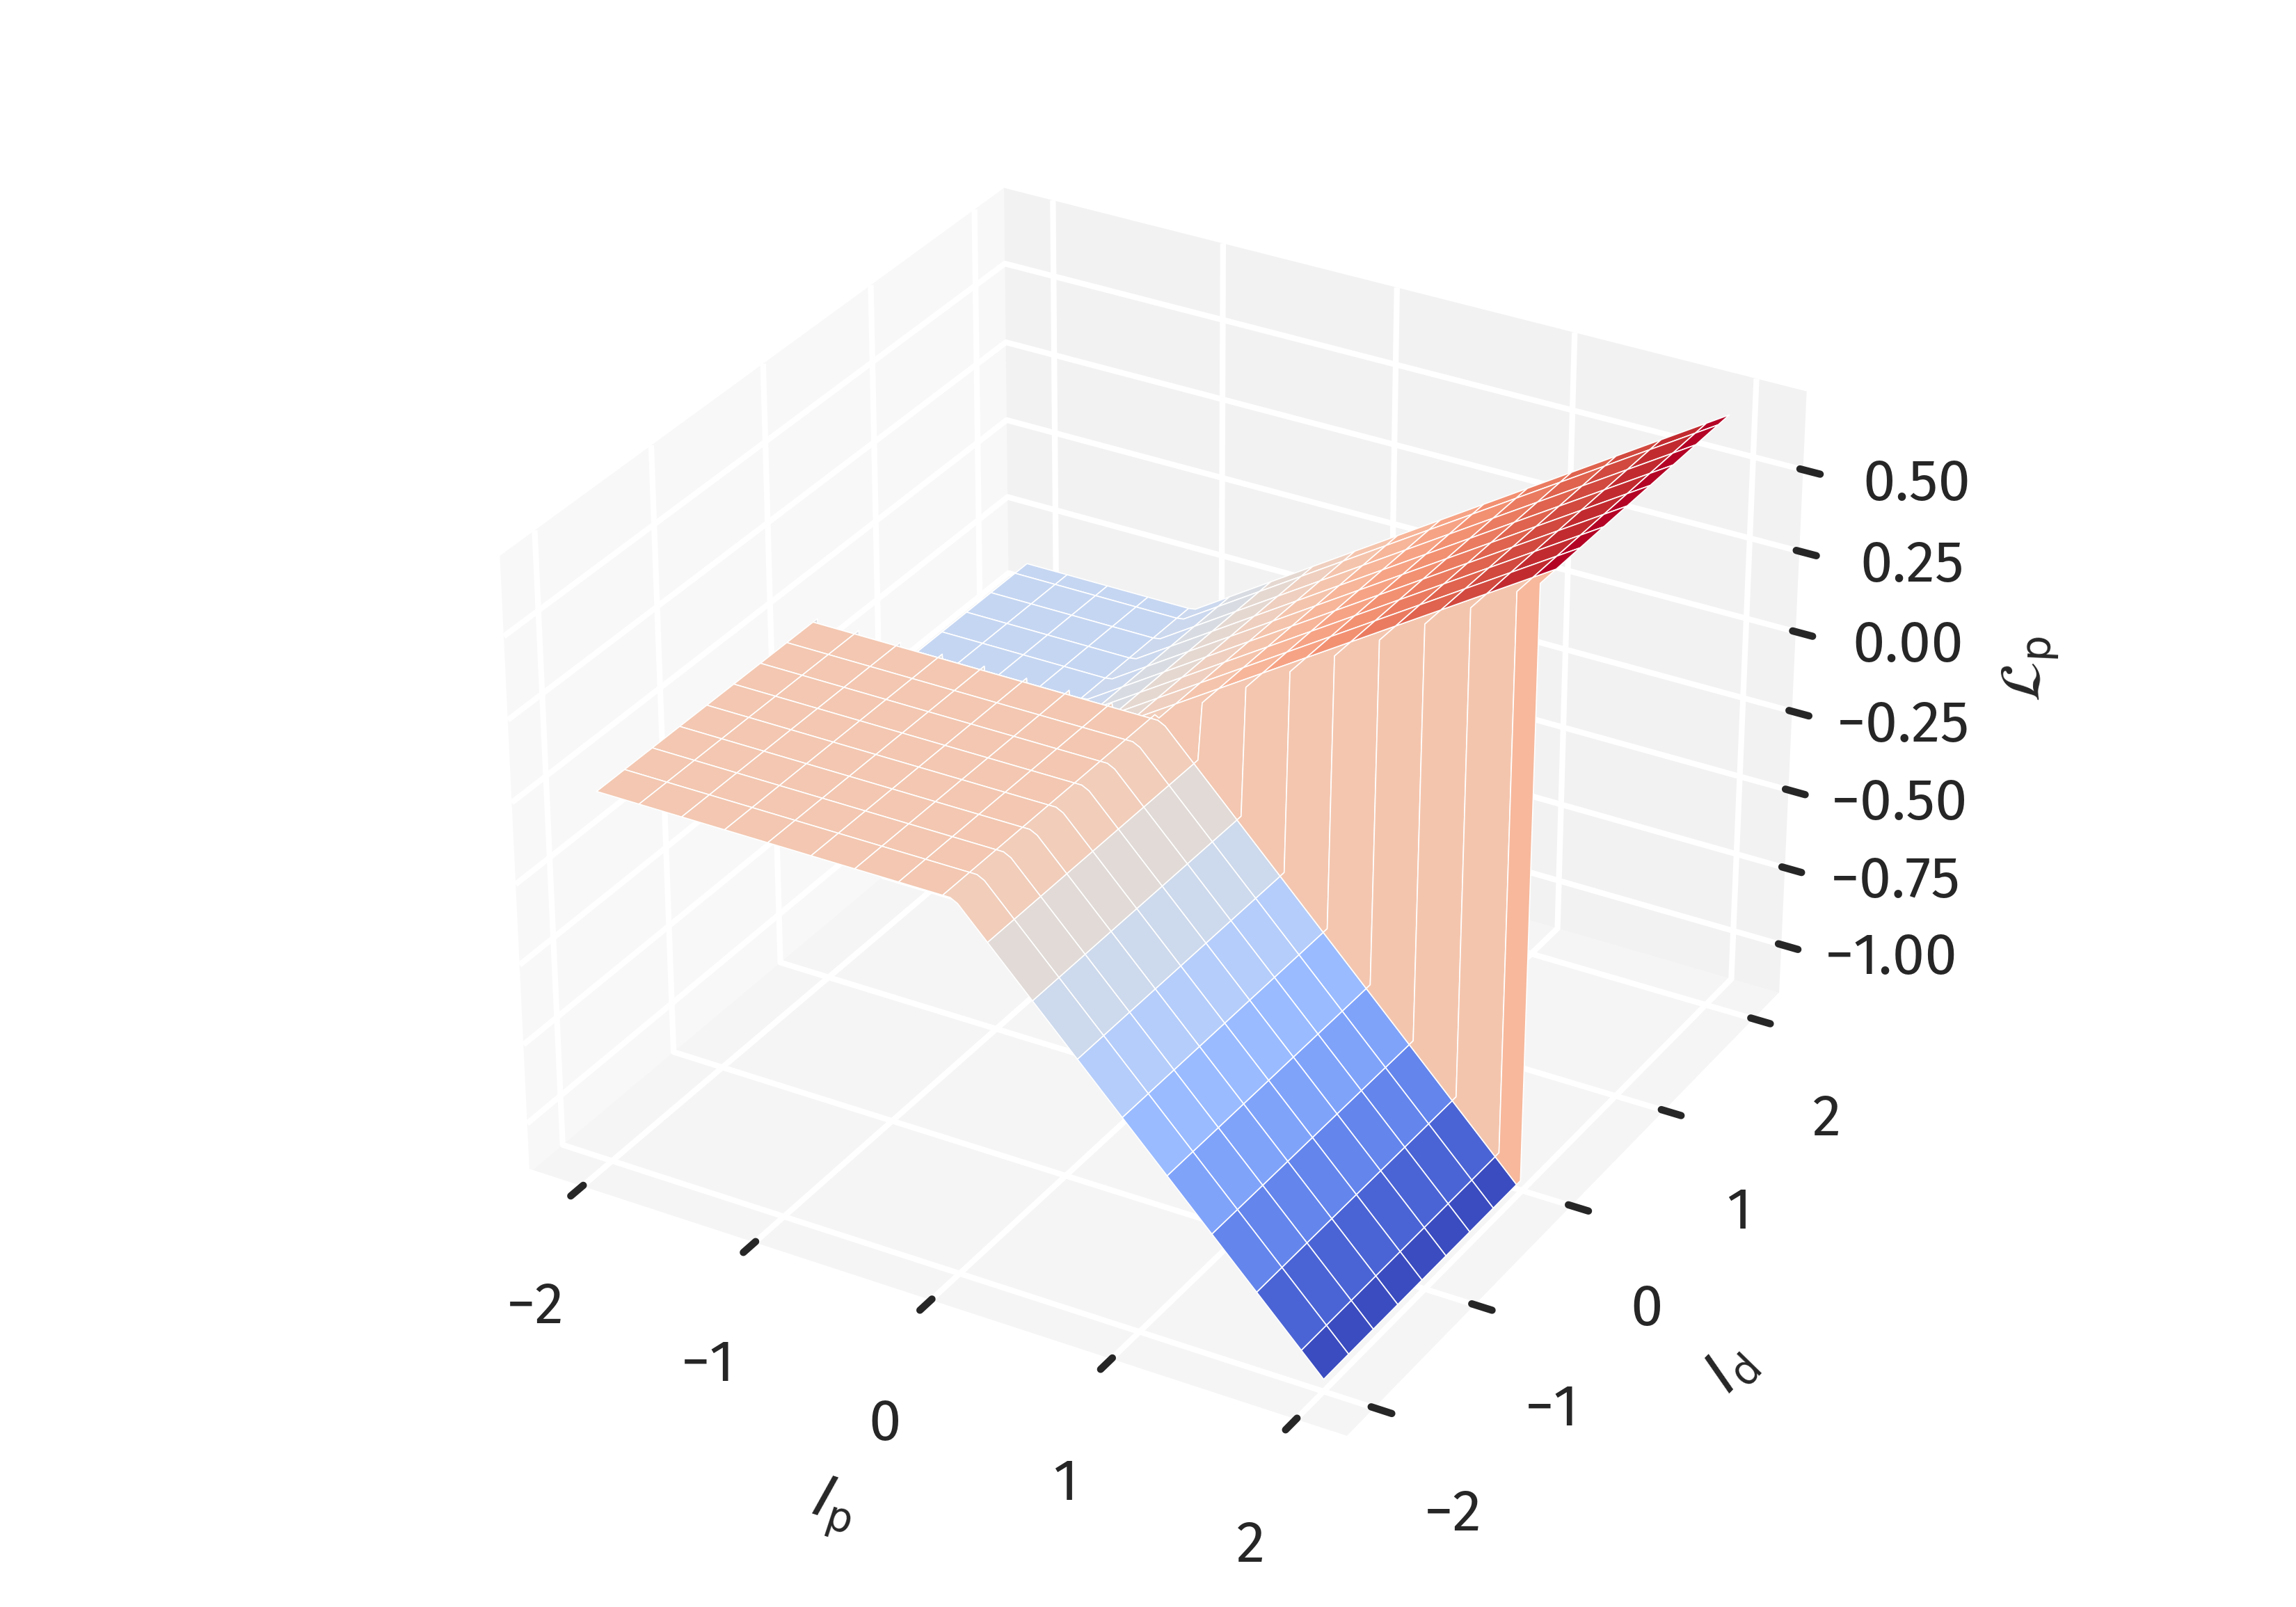
\includegraphics[width=0.7\columnwidth]{obj_func}
\caption{{\bf Objective Function for the Proximal Weight Update.} The 
	approximate objective function for the proximal weights as given in
	\eqref{eq:obj_func}. This corresponds to a combination of using 
	\eqref{eq_comp_model} together with \eqref{eq:bcm_rule}. Note the ridge-like
	structure along the $I_p$-$I_d$ diagonal, which supports the alignment between
	proximal and distal input.}
\label{fig:obj_func}
\end{figure}
%%%%%%%%%%%%%%%%%%%%%%%%%%%%%%%%%%%%%

It should be noted, though, that to a certain extent, the objective 
function is not scale-invariant (as would be e.g.\ if 
the squared error was used) in the sense 
that the prior distributions of both proximal 
and distal inputs need a certain mean and variance to cover a region of input
states for which the described effects can take place. 
As a counterexample, one could imagine that the input samples 
only covered a flat of $\mathcal{L}_p$, as for example in 
Fig.~\ref{fig:obj_func} on the left, leading to a zero average gradient. 
This is prevented, however, by the homeostatic processes 
acting simultaneously on the gains
and biases.

%---------------------------------------%
\section{Discussion}
%---------------------------------------%

We have demonstrated that in a simple supervised learning scheme, the
proposed two-compartment transfer function significantly increases
the robustness of the learning process against distracting components
in the proximal input space. This was most prominently found when
combined with a BCM-like learning rule.

The idea of target-backpropagation in multi-layered networks
has already been proposed in different variants
\citep{Bengio2014,Lee2015,Guerguiev2017}. Yet, all of these approaches
assume a learning rule being dependent on an explicit error term 
between top-down and bottom up signals guiding plasticity in some form
or another. In this work, we considered an alternative approach, that is,
the correlation between proximal and distal input as a maximization
objective, in combination with homeostatic adaptation rules that regulate
proximal and distal inputs into a desired ``working regime'', 
see Sect.~\ref{sect:Obj_Func}. 
Since $I_p$ is a linear projection of the 
proximal input space, maximizing the correlation between
$I_p$ and $I_d$ can be regarded as a form of canonical correlation
analysis (CCA) \citep{Haerdle2007}. The idea of investigating CCA as a
possible mode of synaptic learning has previously been investigated by
\citet{Haga2018}. Interestingly, according to the authors, a 
BCM-learning term in the plasticity dynamics accounts for principal component
analysis in the input space, while CCA requires an additional multiplicative
term between local basal and apical activity. In contrast, our results
indicate that such a multiplicative term is not required to drive basal
synaptic plasticity towards a maximal alignment between basal and apical
input, even in the presence of distracting principal components.
Apart from the advantage that this avoids the necessity of giving
a biophysical interpretation of such cross-terms, it is also in line
with the view that synaptic plasticity should be formulated
in terms of local membrane voltage traces \citep{Clopath2010,Weissenberger2018}. 
Distal compartments then only implicitly affect plasticity, 
e.g.\ by facilitating spike initiation.

As we did not include higher-dimensional distal input patterns, it
remains an open question how target signals would be formed in
multi-layered network structures. However, as previous works have
indicated, random top-down weights can be sufficient for
successful credit assignment and learning \citep{Lillicrap2016,Guerguiev2017}.
Therefore, our results could potentially also be transferred to deeper
network structures, where plasticity is guided by local errors between
top-down and bottom-up signals.

%---------------------------------------%
\section{Supplementary Material}
%---------------------------------------%
%%%%%%%%%%%%%%%%%%%%%%%%%%%%%%%%%%%%%
\begin{figure}[t]
\centering
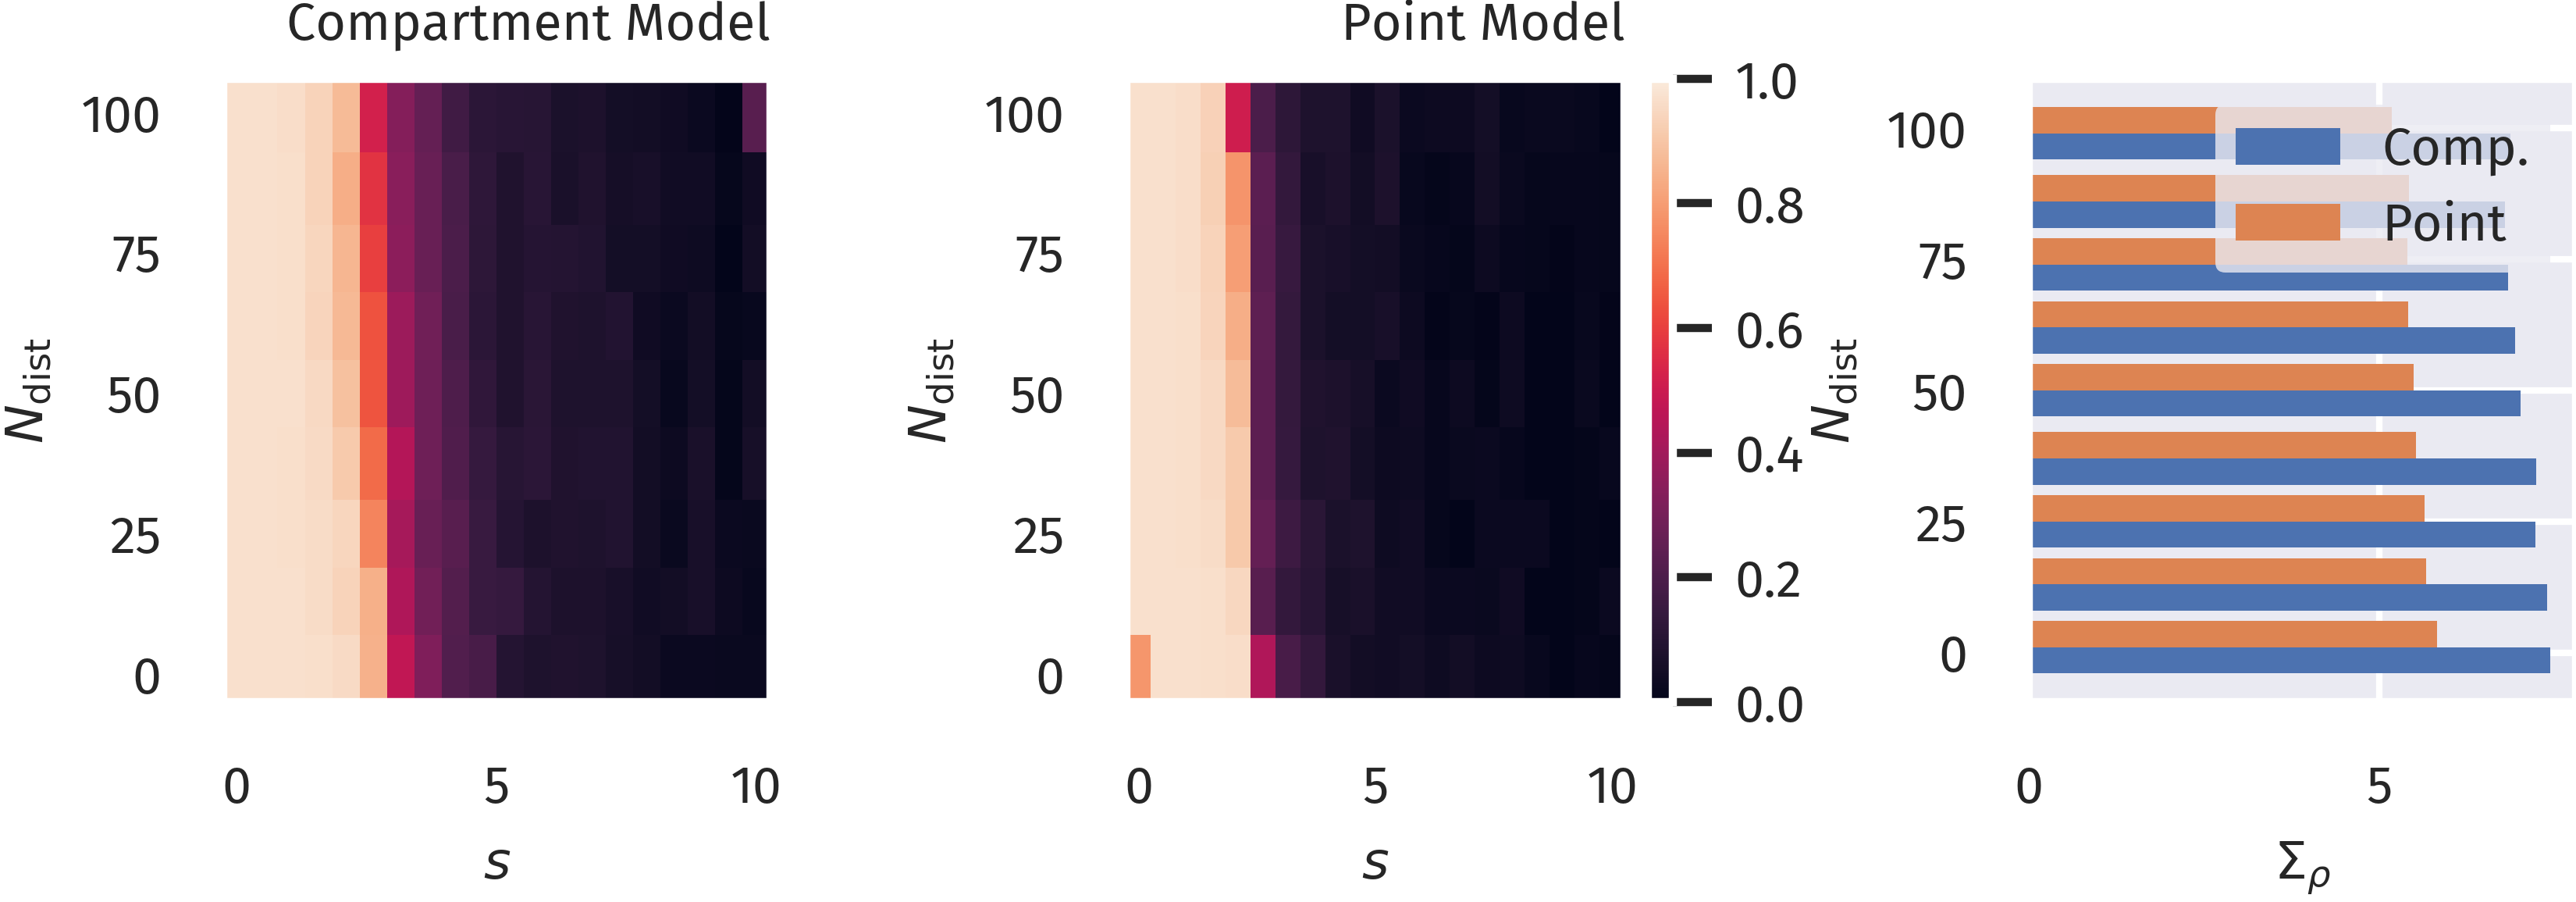
\includegraphics[width=1.0\columnwidth]{classification_correlation_dimension_scaling_high_input_dim}
\caption{{\bf Alignment between Basal and Apical Input after Binary Classification Learning.}
	Correlation between proximal and distal Input after training as described in 
	Sect.~\ref{sect:classification}. The quantity $\Sigma_{\rho}$ depicted in the bar
	plot is the sum over all correlation values for the different tested values
	of $s$ under a given $N_{\rm dist}$. Blue bar represents the compartment model,
	orange the point model.}
\label{fig:classification_correlation}
\end{figure}
%%%%%%%%%%%%%%%%%%%%%%%%%%%%%%%%%%%%%

%%%%%%%%%%%%%%%%%%%%%%%%%%%%%%%%%%%%%
\begin{figure}[t]
\centering
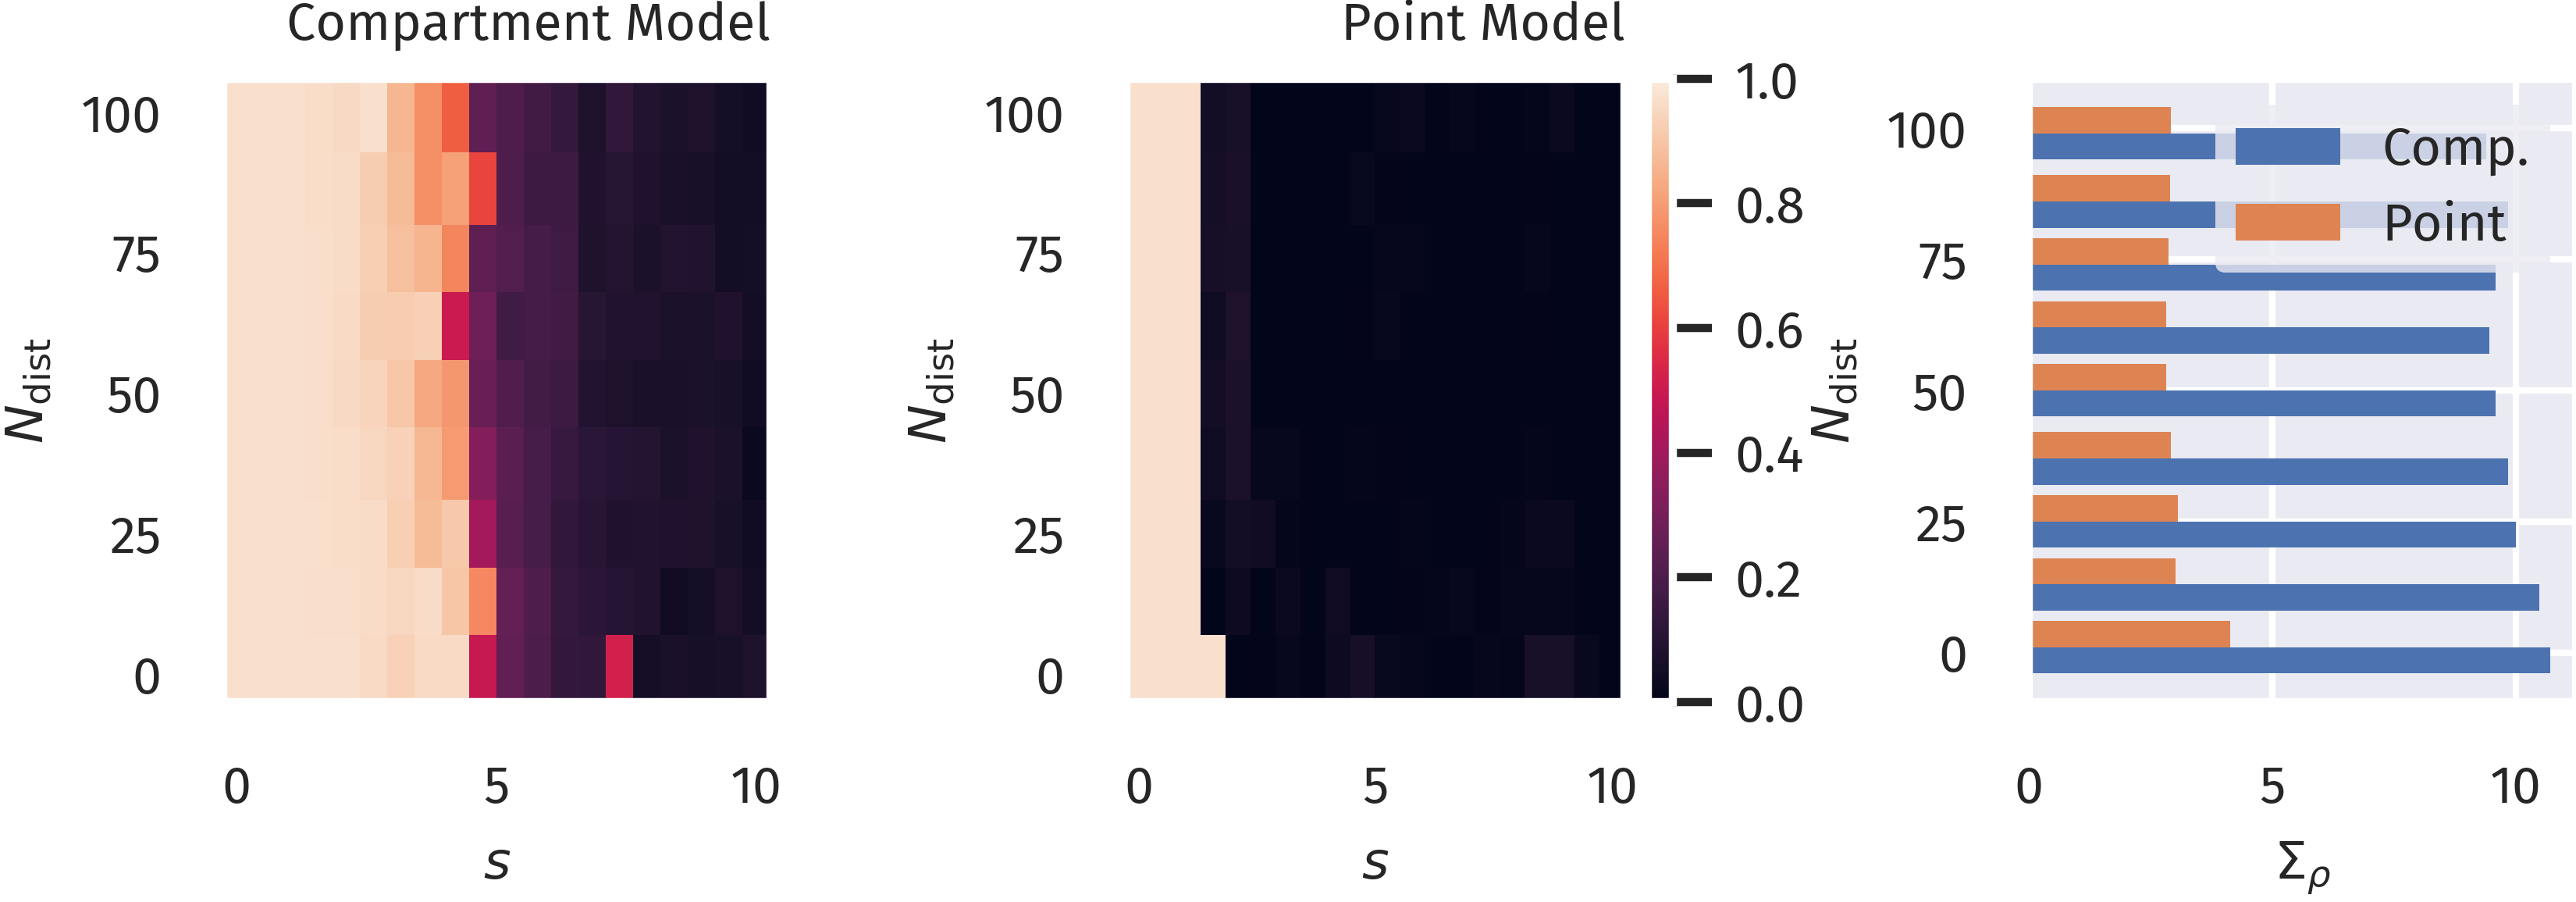
\includegraphics[width=1.0\columnwidth]{classification_correlation_dimension_scaling_bcm_high_input_dim}
\caption{{\bf Alignment between Basal and Apical Input after Binary Classification Learning
		using a BCM-like Rule.}
	Correlation between proximal and distal Input after linear classification 
	training as described in Sect.~\ref{sect:classification}, but using the plasticity
	rules given in Sect.~\ref{sect:non-hebbian}. The quantity $\Sigma_{\rho}$ depicted in the bar
	plot is the sum over all correlation values for the different tested values
	of $s$ under a given $N_{\rm dist}$. Blue bar represents the compartment model,
	orange the point model.}
\label{fig:classification_correlation_bcm}
\end{figure}
%%%%%%%%%%%%%%%%%%%%%%%%%%%%%%%%%%%%%

%\section{Manuscript Formatting}
%
%\subsection{Heading Levels}
%
%%There are 5 heading levels
%
%\subsection{Level 2}
%\subsubsection{Level 3}
%\paragraph{Level 4}
%\subparagraph{Level 5}
%
%\subsection{Equations}
%Equations should be inserted in editable format from the equation editor.
%
%\begin{equation}
%\sum x+ y =Z\label{eq:01}
%\end{equation}
%
%\subsection{Figures}
%Frontiers requires figures to be submitted individually, in the same order as they are referred to in the manuscript. Figures will then be automatically embedded at the bottom of the submitted manuscript. Kindly ensure that each table and figure is mentioned in the text and in numerical order. Figures must be of sufficient resolution for publication \href{http://home.frontiersin.org/about/author-guidelines#ResolutionRequirements}{see here for examples and minimum requirements}. Figures which are not according to the guidelines will cause substantial delay during the production process. Please see \href{http://home.frontiersin.org/about/author-guidelines#GeneralStyleGuidelinesforFigures}{here} for full figure guidelines. Cite figures with subfigures as figure \ref{fig:2}B.
%
%
%\subsubsection{Permission to Reuse and Copyright}
%Figures, tables, and images will be published under a Creative Commons CC-BY licence and permission must be obtained for use of copyrighted material from other sources (including re-published/adapted/modified/partial figures and images from the internet). It is the responsibility of the authors to acquire the licenses, to follow any citation instructions requested by third-party rights holders, and cover any supplementary charges.
%%%Figures, tables, and images will be published under a Creative Commons CC-BY licence and permission must be obtained for use of copyrighted material from other sources (including re-published/adapted/modified/partial figures and images from the internet). It is the responsibility of the authors to acquire the licenses, to follow any citation instructions requested by third-party rights holders, and cover any supplementary charges.
%
%\subsection{Tables}
%Tables should be inserted at the end of the manuscript. Please build your table directly in LaTeX.Tables provided as jpeg/tiff files will not be accepted. Please note that very large tables (covering several pages) cannot be included in the final PDF for reasons of space. These tables will be published as \href{http://home.frontiersin.org/about/author-guidelines#SupplementaryMaterial}{Supplementary Material} on the online article page at the time of acceptance. The author will be notified during the typesetting of the final article if this is the case. 
%
%\section{Nomenclature}
%
%\subsection{Resource Identification Initiative}
%To take part in the Resource Identification Initiative, please use the corresponding catalog number and RRID in your current manuscript. For more information about the project and for steps on how to search for an RRID, please click \href{http://www.frontiersin.org/files/pdf/letter_to_author.pdf}{here}.
%
%\subsection{Life Science Identifiers}
%Life Science Identifiers (LSIDs) for ZOOBANK registered names or nomenclatural acts should be listed in the manuscript before the keywords. For more information on LSIDs please see \href{http://www.frontiersin.org/about/AuthorGuidelines#InclusionofZoologicalNomenclature}{Inclusion of Zoological Nomenclature} section of the guidelines.
%
%
%\section{Additional Requirements}
%
%For additional requirements for specific article types and further information please refer to \href{http://www.frontiersin.org/about/AuthorGuidelines#AdditionalRequirements}{Author Guidelines}.

\section*{Conflict of Interest Statement}
%All financial, commercial or other relationships that might be perceived by the academic community as representing a potential conflict of interest must be disclosed. If no such relationship exists, authors will be asked to confirm the following statement: 

The authors declare that the research was conducted in the absence of any commercial or financial relationships that could be construed as a potential conflict of interest.

\section*{Author Contributions}

Both authors, F.S. and C.G., contributed equally to the
writing and review of the manuscript. F.S. provided the code,
ran the simulations and prepared the figures.

%\section*{Funding}
%Details of all funding sources should be provided, including grant numbers if applicable. Please ensure to add all necessary funding information, as after publication this is no longer possible.

%---------------------------------------%
\section*{Acknowledgments}
%---------------------------------------%

The authors acknowledge the financial support of
the German research foundation (DFG)
%\section*{Supplemental Data}
% \href{http://home.frontiersin.org/about/author-guidelines#SupplementaryMaterial}{Supplementary Material} 
% should be uploaded separately on submission, if there are Supplementary Figures, 
% please include the caption in the same file as the figure. LaTeX Supplementary Material templates can be found in the Frontiers LaTeX folder.

\section*{Data Availability Statement}
The datasets [GENERATED/ANALYZED] for this study can be found in the [NAME OF REPOSITORY] [LINK].
% Please see the availability of data guidelines for more information, 
%at https://www.frontiersin.org/about/author-guidelines#AvailabilityofData

\bibliographystyle{frontiersinSCNS_ENG_HUMS} % for Science, Engineering and Humanities 
%and Social Sciences articles, for Humanities and Social 
%Sciences articles please include page numbers in the in-text citations
%\bibliographystyle{frontiersinHLTH&FPHY} % for Health, 
%Physics and Mathematics articles
\bibliography{Dendritic_Learning.bib}

%%% Make sure to upload the bib file along with the tex file and PDF
%%% Please see the test.bib file for some examples of references

%\section*{Figure captions}
%
%%%% Please be aware that for original research articles we only permit 
%%a combined number of 15 figures and tables, one figure with multiple 
%%subfigures will count as only one figure.
%%%% Use this if adding the figures directly in the mansucript, if so, 
%%please remember to also upload the files when submitting your article
%%%% There is no need for adding the file termination, as long as 
%%you indicate where the file is saved. In the examples below the 
%%files (logo1.eps and logos.eps) are in the Frontiers LaTeX folder
%%%% If using *.tif files convert them to .jpg or .png
%%%%  NB logo1.eps is required in the path in order to correctly 
%%compile front page header %%%
%
%\begin{figure}[h!]
%\begin{center}
%
\includegraphics[width=10cm]{logo1}% This is a *.eps file
%\end{center}
%\caption{ Enter the caption for your figure here.  Repeat as  necessary for each of your figures}\label{fig:1}
%\end{figure}
%
%
%\begin{figure}[h!]
%\begin{center}
%\includegraphics[width=15cm]{logos}
%\end{center}
%\caption{This is a figure with sub figures, \textbf{(A)} is one logo, \textbf{(B)} is a different logo.}\label{fig:2}
%\end{figure}
%
%%%% If you are submitting a figure with subfigures please combine these into one image file with part labels integrated.
%%%% If you don't add the figures in the LaTeX files, please upload them when submitting the article.
%%%% Frontiers will add the figures at the end of the provisional pdf automatically
%%%% The use of LaTeX coding to draw Diagrams/Figures/Structures should be avoided. They should be external callouts including graphics.

\end{document}
